\textbf{8.1.1.} 法拉第电磁感应定律为 $\varepsilon = -\frac{d\Phi}{dt}$ . 有人说: (1) 这个式子不是法拉第提出来的; (2) 式中的负号是人为规定的结果. 你认为这个人说的两点是对的还是错的?

\vfill

\textbf{8.1.2.} 感应电动势 $\mathcal{E}$ 是标量, 不是矢量, 通常说: “感应电动势的方向” 是什么意思? 对于一个导线回路, 如何由 $\varepsilon = -\frac{\mathrm{d}\Phi}{\mathrm{d}t}$ 确定 $\mathcal{E}$ 的方向?

【解答】感应电动势的方向是指它的非静电力 $(E_{i})$ 的方向.

确定 $\mathcal{E}$ 的方向的方法如下：沿回路 $L$ 任意规定一个绕行方向，即线元 $\mathrm{d}l$ 的方向，以此绕行方向的右旋进方向为回路 $L$ 的法线方向 $\pmb{n}$ ，如图8.1.2所示，则有

$$
\ell = \oint_ {L} \boldsymbol {E} _ {i} \cdot \mathrm{d} \boldsymbol {l} = - \frac {\mathrm{d}}{\mathrm{d} t} \iint_ {S} \boldsymbol {B} \cdot \boldsymbol {n} \mathrm{d} S
$$

若 $-\frac{\mathrm{d}}{\mathrm{d}t}\iint_{S}\pmb {B}\cdot \pmb {n}\mathrm{d}S > 0$ ，则 $\varepsilon >0$ ，即 $\varepsilon$ 与 $\mathrm{d}l$ 方向相同；若 $-\frac{\mathrm{d}}{\mathrm{d}t}\iint_{S}\pmb {B}\cdot \pmb {n}\mathrm{d}S < 0$ ，则 $\varepsilon < 0$ ，即 $\varepsilon$ 与 $\mathrm{d}l$ 方向相反.

\vfill

\newpage

\textbf{8.1.3.} 法拉第电磁感应定律为 $\varepsilon = -\frac{d\Phi}{dt}$ ，试说明式中的负号表示楞次定律.

【解答】在磁通量 $\Phi = \iint_{S} \mathbf{B} \cdot \mathrm{d}\mathbf{S}$ 和感应电动势 $\mathcal{E} = \oint_{L} \mathbf{E}_i \cdot \mathrm{d}\mathbf{l}$ 这两个定义式中，面积元 $\mathrm{d}\mathbf{S} = \mathbf{n}\mathrm{d}\mathbf{S}$ 的方向规定为 $\mathrm{d}\mathbf{l}$ 的右旋进方向，如图8.1.3(1)所示。在这种规定下， $\mathcal{E} = -\frac{\mathrm{d}\Phi}{\mathrm{d}t}$ 中的负号便表示楞次定律，说明如下：

(1)

(2)
图8.1.3

(3)

如图8.1.3(2)，取 $\pmb{n}$ 与 $\pmb{B}$ 的夹角小于 $90^{\circ}$ ，则 $\mathrm{d}l$ 便按规定为 $\pmb{n}$ 的右手螺旋方向。这时 $\Phi = \iint_{S} \pmb{B} \cdot \mathrm{d}\pmb{S} > 0$ 。若 $\pmb{B}$ 增大， $\Phi$ 也增大，故 $\frac{\mathrm{d}\Phi}{\mathrm{d}t} > 0$ ， $\varepsilon = \oint_{L} \pmb{E}_i \cdot \mathrm{d}l = -\frac{\mathrm{d}\Phi}{\mathrm{d}t} < 0$ ，所以 $\pmb{E}_i$ 与 $\mathrm{d}l$ 方向相反。若 $\pmb{B}$ 减小， $\Phi$ 也减小，故 $\frac{\mathrm{d}\Phi}{\mathrm{d}t} < 0$ ， $\varepsilon = \oint_{L} \pmb{E}_i \cdot \mathrm{d}l = -\frac{\mathrm{d}\Phi}{\mathrm{d}t} > 0$ ，所以 $\pmb{E}_i$ 与 $\mathrm{d}l$ 方向相同。可见负号表示了楞次定律所规定的 $\pmb{E}_i$ 的方向，即感应电流的方向。

如果取 n 与 B 的夹角大于 $90^{\circ}$ ，如图 8.1.3(3) 所示，dl 按规定仍为 n 的右手螺旋方向。这时 $\Phi = \iint_{S} B \cdot dS < 0$ 。若 B 增大， $\Phi$ 便减小，故 $\frac{d\Phi}{dt} < 0$ ， $\varepsilon = \oint_{L} E_{i} \cdot dl = -\frac{d\Phi}{dt} > 0$ ，所以 $E_{i}$ 与 dl 方向相同。若 B 减小， $\Phi$ 便增大，故 $\frac{d\Phi}{dt} > 0$ ， $\varepsilon = \oint_{L} E_{i} \cdot dl = -\frac{d\Phi}{dt} < 0$ ，所以 $E_{i}$ 与 dl 方向相反。

由以上分析可见,不论是哪种情况,只要规定了 n 为 dl 的右旋进方向,则 $\varepsilon = -\frac{d\Phi}{dt}$ 中的负号就表示了 $E_{j}$ 的方向,即楞次定律所规定的方向.
\begin{center}
    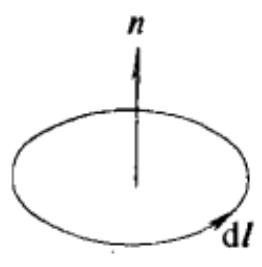
\includegraphics[width=0.5\linewidth]{figures/fig_8_1_3_1.jpg}
\end{center}
\begin{center}
    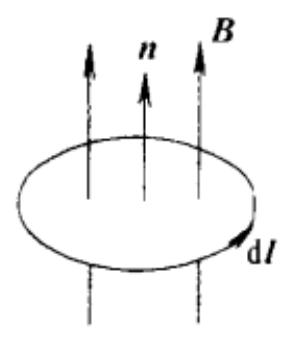
\includegraphics[width=0.5\linewidth]{figures/fig_8_1_3_2.jpg}
\end{center}
\begin{center}
    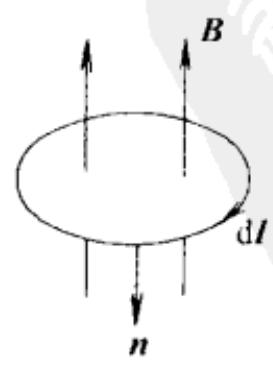
\includegraphics[width=0.5\linewidth]{figures/fig_8_1_3_3.jpg}
\end{center}

\vfill

\textbf{8.1.4.} 试用简单的例子说明,楞次定律是能量守恒所必须的.换句话说,如果电磁感应的规律正好与楞次定律相反,则能量守恒定律便不成立.

【解答】如图8.1.4,外力 $\pmb{F}$ 作用在磁棒上，使它的N极向线圈运动；根据楞次定律，线圈里产生感应电流 $I_{i}, I_{i}$ 的磁场反抗磁棒N极向线圈的运动。因此，要使磁棒向线圈运动，外力必须反抗 $I_{i}$ 的磁场作功。这功的能量就转化成线圈电流所产生的焦耳热。

图8.1.4

如果电磁感应的规律正好与楞次定律相反，即 $I_{i}$ 的方向与图8.1.4中的相反，则 $I_{i}$ 的磁场作用在磁棒上的力便是吸引力，使之向线圈加速运动。这样， $I_{i}$ 便对磁棒作功，同时还产生焦耳热。于是能量守恒定律便不成立了。
\begin{center}
    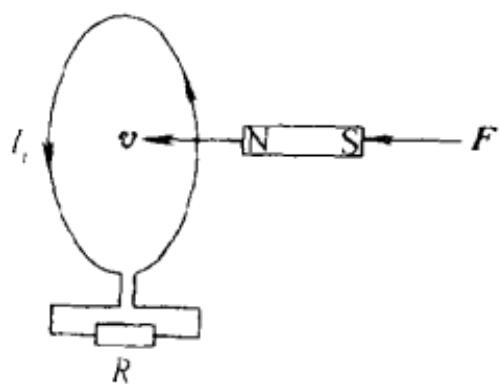
\includegraphics[width=0.5\linewidth]{figures/fig_8_1_4.jpg}
\end{center}

\vfill

\newpage

\textbf{8.1.5.} 试证明 $\frac{\mathrm{d}\Phi}{\mathrm{d}t}$ 的单位为伏特.

\vfill

\textbf{8.1.6.} 试评论下列几种说法:(1)感应电动势的方向是指感应电场的电场强度(非静电力)的方向；(2)在一个线圈里，感应电动势的方向是指其中电流的方向；(3)在磁场变化所产生的感应电场中，两点的电势差是没有意义的；(4)导体处在磁场变化所产生的电场中，它上面两点的电势差是没有意义的.

【解答】（1）和(3)都是对的.

(2)不对.由于还可能有其他原因(如电池)产生电流,线圈里电流的方向不一定与感应电动势的方向相同;还有,线圈若不构成闭合回路,其中便没有电流,但仍可有感应电动势存在.

(4)不对.感应电场 $E_{i}$ 使导体内的自由电荷运动，结果在导体表面上产生电荷，这电荷产生静电场 $\pmb{E}_{s}$ ，使得导体内 $E_{i} + E_{s} = 0$ ，达到平衡。由于静电场的存在，导体上面两点的电势差便是这静电场的电势差，是有意义的。


图8.1.7
\begin{center}
    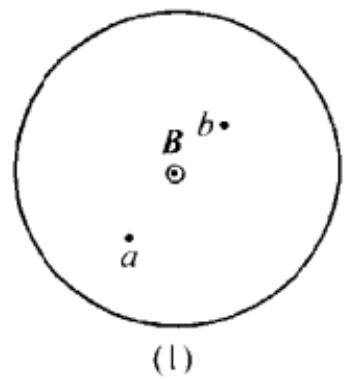
\includegraphics[width=0.5\linewidth]{figures/fig_8_1_6_1.jpg}
\end{center}
\begin{center}
    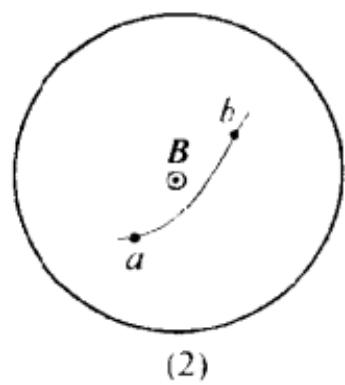
\includegraphics[width=0.5\linewidth]{figures/fig_8_1_6_2.jpg}
\end{center}

\vfill

\newpage

\textbf{8.1.7.} 在一圆柱形空间里有均匀磁场，磁感强度 B 平行于轴线，其横截面如图 8.1.7(1) 所示。当 B 的大小发生变化时，空间两点 a、b 间有电势差吗？如果在这磁场中放一根导线，使其经过 a、b 两点，如图 8.1.7(2) 所示。这时导线上的 a、b 两点有电势差吗？

【解答】在图8.1.7(1)中， $\pmb{B}$ 的大小变化所产

生的感应电场 $E_{i}$ 是涡旋电场，对这种电场是不能定义电势的。因此，图8.1.7(1)中，“a、b两点的电势差”是没有意义的。

如果在其中放一根通过 $a, b$ 两点的导线，则这导线上 $a, b$ 两点的电势差便有意义。这时导线上 $a, b$ 两点的电势差就是涡旋电场 $\pmb{E}_i$ 使导线两端或其他地方出现电荷所产生的静电场（或稳恒电场）的电势差。

\vfill

\textbf{8.1.8.} 磁场变化产生的感应电场是涡旋电场,对于这种电场,是不能定义电势的.为什么处在这电场中的导体上不同地方可以有电势差呢?

【解答】处在感应电场中的导体就成为一个电源，导体内的感应电场的电场强度 $E_{i}$ 就是这电源的非静电力，它驱使导体内的自由电子往 $E_{i}$ 的反方向运动。从而使导体上有的地方出现正电荷，有的地方出现负电荷，这些电荷产生的电场是静电场或稳恒电场，导体上不同地方的电势差就是这种电场的电势差，而不是感应电场的电势差。感应电场是不能定义电势的。

\vfill

\newpage

\textbf{8.1.9.} 导体在磁场中运动时,它里面的自由电子因受到洛伦兹力的作用,从而产生感应电流,可以对外作功.但洛伦兹力是不作功的.那么,感应电流对外作功的能量是从哪里来的呢?试说明原因.

【解答】如图8.1.9(1)，导体在外力 $\pmb{F}$ 的作用下，以速度 $v$ 在磁感强度为 $\pmb{B}$ 的磁场中运动， $\pmb{B}$ 垂直于纸面向外。在 $\pmb{B}$ 的作用下，导体里的自由电子以平均定向速度 $\pmb{u}$ 相对于导体运动。这样，自由电子的速度便为 $u + v$ ，它所受的洛伦兹力为

$$
\boldsymbol {f} = - e (\boldsymbol {u} + \boldsymbol {v}) \times \boldsymbol {B}\tag{1}
$$

$f$ 与 $u + v$ 垂直，故 $f$ 作功的功率为零.

(1)

(2)
图8.1.9

由图8.1.9(2)可见， $f$ 可分解为平行于 $\pmb{u}$ 的分量 $f$ 和垂直于 $\pmb{u}$ 的分量 $f_{-}$ ，即

$$
\boldsymbol {f} = \boldsymbol {f} _ {\text {丨}} + \boldsymbol {f} _ {\text {丿}}\tag{2}
$$

其中 $f_{1}$ 作功的功率为

$$
f _ {\parallel} \cdot (u + v) = f _ {\parallel} \cdot u > 0\tag{3}
$$

$f_{\perp}$ 作功的功率为

$$
f _ {\perp} \cdot (u + v) = f _ {\perp} \cdot v <   0\tag{4}
$$

即 $f_{\parallel}$ 对形成感应电流的自由电子作了正功，而 $f_{\perp}$ 则作了负功，正负功之和为零.

对于运动的导体来说， $f_{\perp}$ 是阻力。因此，使导体运动的外力便要克服阻力 $f_{\perp}$ 而作正功。当导体以匀速 v 运动时， $f_{\perp} = -F$ 。这时外力 F 对导体作的正功便正好等于 $f_{\parallel}$ 对自由电子作的正功。这就表明，外力 F 作功所支出的能量通过洛伦兹力转化为感应电流的能量。所以感应电流对外作功的能量是从使导体运动的外力 F 来的。洛伦兹力 f 起了中介的作用，它的 $f_{\perp}$ 接受了 F

作正功所给予的能量,同时它的 $f_{\parallel}$ 对自由电子作正功,将这部分能量转给了感应电流.
\begin{center}
    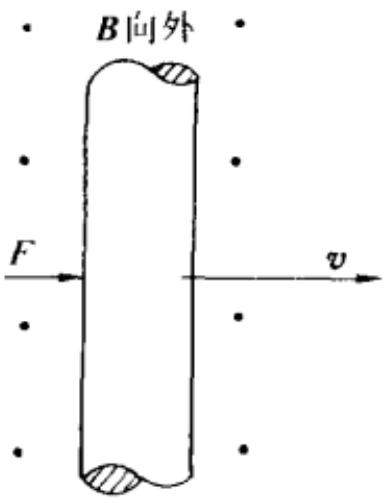
\includegraphics[width=0.5\linewidth]{figures/fig_8_1_9_1.jpg}
\end{center}
\begin{center}
    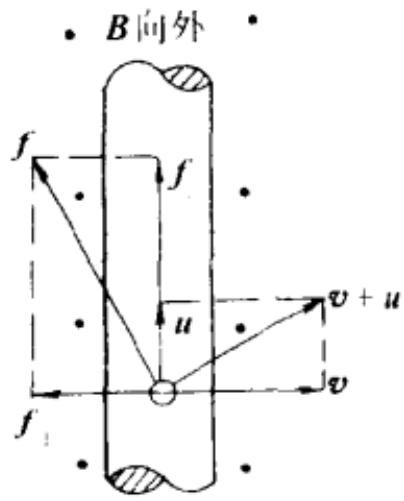
\includegraphics[width=0.5\linewidth]{figures/fig_8_1_9_2.jpg}
\end{center}

\vfill

\textbf{8.1.10.} 法拉第发现电磁感应现象的实验如图 8.1.10 所示: 在一铁环上绕有两组线圈 A 和 B, A 与电池接成回路, B 则自成回路, 它的导线经过一个小磁针的上方. 试问当接通电键 K 时, 小磁针如何运动?

图8.1.10

【解答】K接通时,小磁针上方回路中的感应电流是逆时针方向流动,因此,小磁针的N极向纸面内转动,同时它的S极则向纸面外转动.
\begin{center}
    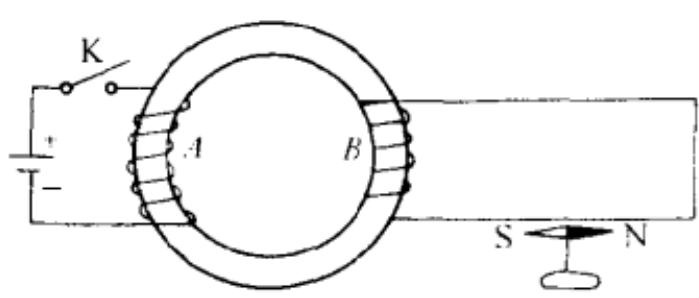
\includegraphics[width=0.5\linewidth]{figures/fig_8_1_10.jpg}
\end{center}

\vfill

\newpage

\textbf{8.1.11.} 一螺线管与电流计 G 联接成闭合回路, 一磁棒与这螺线管平行, 并以速度 v 离开螺线管. 试问电流计 G 中有无电流? 若有电流, 试指出其方向.

【解答】有电流.电流的方向是从 $a$ 经G到 $b$ .

\vfill

\textbf{8.1.12.} 如图 8.1.12, 试判定下列情况下电阻 R 里感应电流的方向: (1) 电流从 a 到 $a'$ 并增大; (2) 电流从 $a'$ 到 a 并减小; (3) 电流从 $a'$ 到 a 并增大.

【解答】(1)从 d 经 R 到 c；(2)从 d 经 R 到 c；(3)从 c 经 R 到 d.

图8.1.11

图8.1.12
\begin{center}
    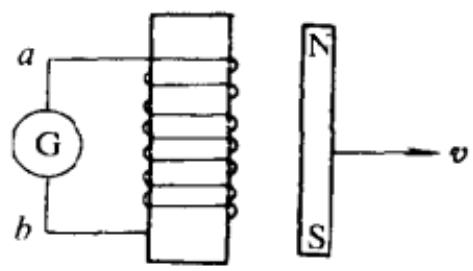
\includegraphics[width=0.5\linewidth]{figures/fig_8_1_12_1.jpg}
\end{center}
\begin{center}
    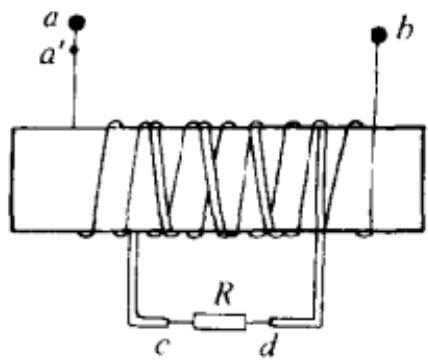
\includegraphics[width=0.5\linewidth]{figures/fig_8_1_12_2.jpg}
\end{center}

\vfill

\newpage

\textbf{8.1.13.} 两个变压器联接如图 8.1.13, 当线圈 A 中的电流 I 增大时, 试指出线圈 B 中感应电动势的方向(即非静电力的方向).

【解答】从 $c$ 到 $d$ .

图8.1.13
\begin{center}
    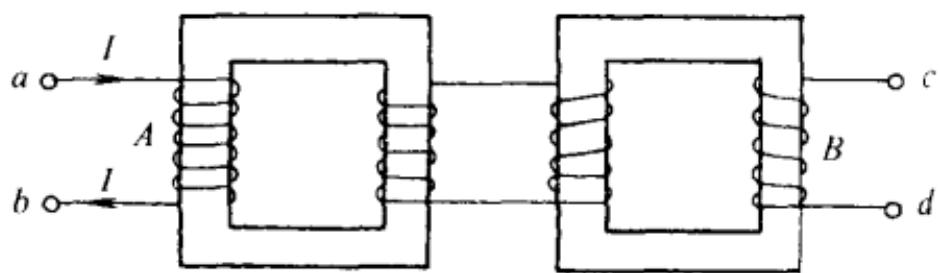
\includegraphics[width=0.5\linewidth]{figures/fig_8_1_13.jpg}
\end{center}

\vfill

\textbf{8.1.14.} 圆环 A 均匀地带有负电荷, 在它外面有一和它共面的金属圆环 B. 现在让 A 环绕它的几何轴旋转, 要在 B 环中产生逆时针方向的电流 I, 如图 8.1.14 所示. 试问 A 环应如何旋转?

【解答】逆时针方向旋转且转速越来越快.或者,顺时针方向旋转且转速越来越慢.

图8.1.14

图8.1.15
\begin{center}
    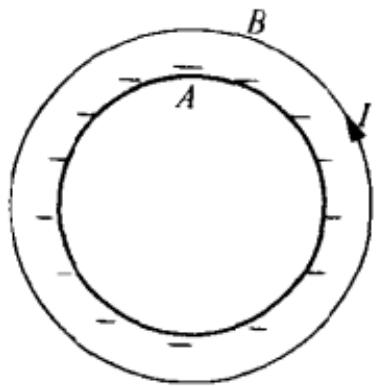
\includegraphics[width=0.5\linewidth]{figures/fig_8_1_14_1.jpg}
\end{center}
\begin{center}
    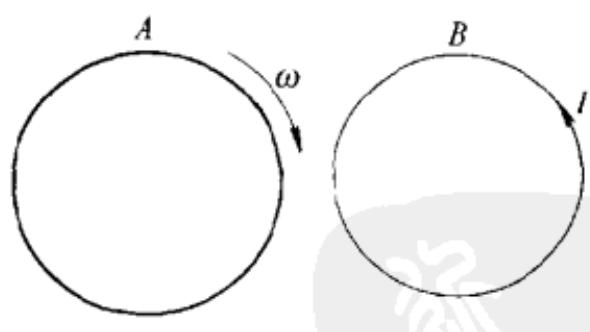
\includegraphics[width=0.5\linewidth]{figures/fig_8_1_14_2.jpg}
\end{center}

\vfill

\newpage

\textbf{8.1.15.} 两个导体圆环 A 和 B 在同一平面内, A 带有电荷, 并绕它的几何轴顺时针旋转, B 则静止不动; 现观测到 B 中有逆时针方向的电流, 如图 8.1.15 所示. 试问 A 带的是正电荷还是负电荷? 它的转动状态如何?

【解答】A 带正电荷, 转速越来越慢. 或者, A 带负电荷, 转速越来越快.

\vfill

\textbf{8.1.16.} 一金属圆环 $A$ 带负电荷, 绕它的几何轴顺时针方向转动; 另外两个金属圆环 $B$ 和 $C$ , 与它在同一平面内, 如图 8.1.16 所示. 当 $A$ 的转速越来越快时, 试问 $B, C$ 两环内感应电流的方向各如何?


图8.1.16


【解答】B、C两环内的感应电流都是逆时针方向.
\begin{center}
    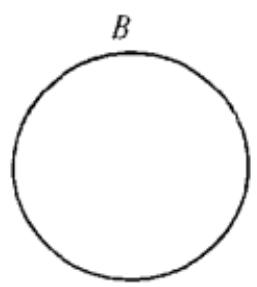
\includegraphics[width=0.5\linewidth]{figures/fig_8_1_16_1.jpg}
\end{center}
\begin{center}
    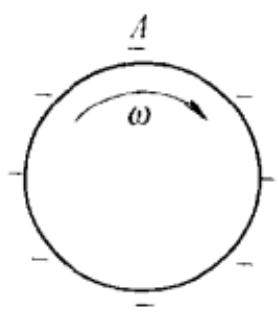
\includegraphics[width=0.5\linewidth]{figures/fig_8_1_16_2.jpg}
\end{center}
\begin{center}
    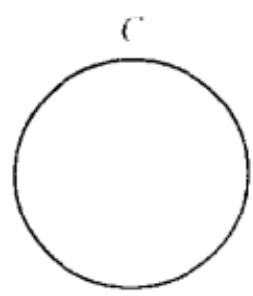
\includegraphics[width=0.5\linewidth]{figures/fig_8_1_16_3.jpg}
\end{center}

\vfill

\newpage

\textbf{8.1.17.} 为了减少涡流损耗,变压器一般都是用表面绝缘的硅钢片作铁芯的.一变压器的外形如图8.1.17所示,试问它的铁芯的硅钢片平行于哪个面?

【解答】硅钢片平行于 DCGE 平面.

图8.1.17

(1)

(2)

(3)
图8.1.18
\begin{center}
    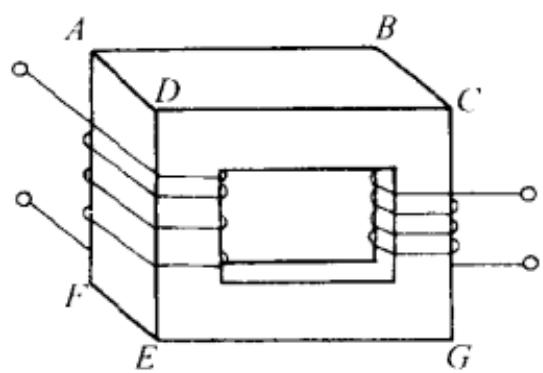
\includegraphics[width=0.5\linewidth]{figures/fig_8_1_17_1.jpg}
\end{center}
\begin{center}
    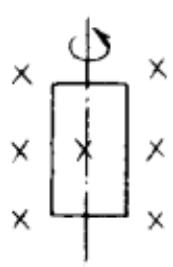
\includegraphics[width=0.5\linewidth]{figures/fig_8_1_17_2.jpg}
\end{center}
\begin{center}
    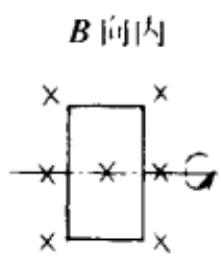
\includegraphics[width=0.5\linewidth]{figures/fig_8_1_17_3.jpg}
\end{center}
\begin{center}
    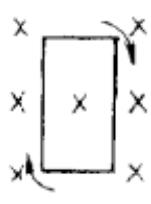
\includegraphics[width=0.5\linewidth]{figures/fig_8_1_17_4.jpg}
\end{center}

\vfill

\textbf{8.1.18.} 矩形线圈在磁感强度为 B 的均匀外磁中转动, 转轴通过线圈中心, 如图 8.1.18 所示. 转轴: (1) 与 B 垂直并与长边平行; (2) 与 B 垂直并与短边平行; (3) 与 B 平行并与线圈平面垂直. 试指出上述三种情况下线圈中感应电流的方向.

【解答】在图8.1.18所示的时刻，(1)和(2)中的线圈平面正好与 $\pmb{B}$ 垂直， $\frac{\mathrm{d}\Phi}{\mathrm{d}t} = 0$ ，所以这时都没有感应电流；从这个位置转过 $90^{\circ}$ 的过程中，(1)和(2)中的感应电流都是顺时针方向。图中的(3)因为通过线圈的磁通量不变，故无感应电流。

\vfill

\newpage

\textbf{8.1.19.} 图 8.1.19 中磁场的磁感强度 B 垂直于纸面并向内, 磁场中有一段运动的导体细杆, 试问在下列运动状态下, 杆内感应电动势的方向各如何? (1) 以 B 为轴线绕杆的中心转动; (2) 绕杆的中心转动, 轴线与杆垂直并与 B 垂直; (3) 沿长度方向平动, 速度 v 与 B 垂直; (4) 以速度 v 平动, v 与杆垂直并与 B 垂直.

【解答】（1）从中心向两端；(2)无感应电动势；(3)无感应电动势；(4)向上.

\vfill

\textbf{8.1.20.} 两根导体杆 ABCD 和 EFGH, AB 和 EF 部分平行, 相距为 L; CD 和 GH 部分平行, 相距为 l. 两杆处在磁感强度为 B 的均匀磁场中, B 与两杆构成的平面垂直并向内，如图8.1.20所示。另有两导体杆 $ab$ 和 $cd$ ，分别横跨在两平行部分，以速度 $\pmb{V}$ 和 $\pmb{v}$ 平行于导体杆运动。试求闭合回路 $abdc$ 中的感应电动势，并指出感应电流沿 $abdc$ 方向流动的条件。

(1)

(2)

(3)
图8.1.19
(4)

图8.1.20
\begin{center}
    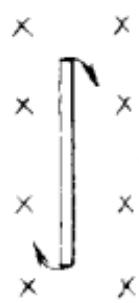
\includegraphics[width=0.5\linewidth]{figures/fig_8_1_20_1.jpg}
\end{center}
\begin{center}
    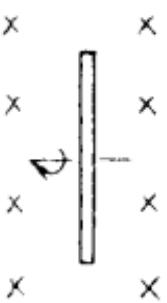
\includegraphics[width=0.5\linewidth]{figures/fig_8_1_20_2.jpg}
\end{center}
\begin{center}
    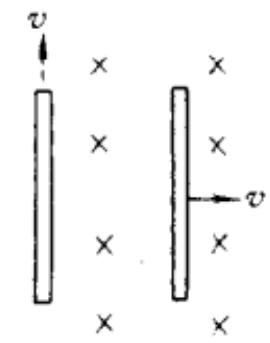
\includegraphics[width=0.5\linewidth]{figures/fig_8_1_20_3.jpg}
\end{center}
\begin{center}
    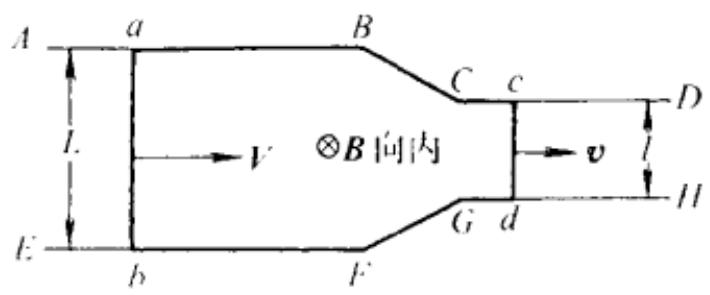
\includegraphics[width=0.5\linewidth]{figures/fig_8_1_20_4.jpg}
\end{center}

\vfill

\newpage

\textbf{8.1.21.} 一矩形导体回路 ABCD 放在均匀外磁场中，磁场的磁感强度 B 的大小为 $B = 6.0 \times 10^{3} G s$ ，B 与矩形平面的法线 n 夹角为 $\alpha = 60^{\circ}$ ; 回路的 CD 段长为 l = 1.0 m, 以速度 v = 5.0 m/s 平行于两边向外滑动, 如图 8.1.21 所示. 试求回路中的感应电动势, 并指出感应电流的方向.

图8.1.21

\vfill

\textbf{8.1.22.} 三条平行导线 AB、CD 和 EF 在同一平面内，AB 和 CD 相距为 $l_{1}$ ，

CD 和 EF 相距为 $l_{2}$ ，A、E 之间以电阻 R 联接，B、D 之间以电阻 r 联接；一条导体杆 ab 横跨在这三条导线上，以匀速 v 在磁感强度为 B 的均匀磁场中滑动，v 平行于三条导线，B 垂直于三条导线所构成的平面并向外，如图 8.1.22 所示。试分别求通过 R 和 r 的电流。

图8.1.22
\begin{center}
    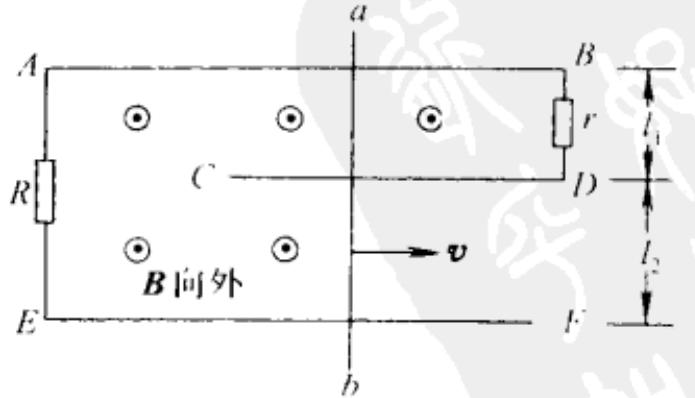
\includegraphics[width=0.5\linewidth]{figures/fig_8_1_22.jpg}
\end{center}

\vfill

\newpage

\textbf{8.1.23.} 两根平行的导线 ab 和 cd，长度都是 l，各有一端与弯成乙形的金属细杆接触，它们都在同一平面内，并处在磁感强度为 B 的均匀磁场中，B 与这平面垂直并向内，如图 8.1.23 所示。试求下列两种情况下 a、d 两端的电势差：(1) 细杆和两导线都以速度 v (v

图8.1.23

与导线垂直)运动；(2)细杆不动，两导线都以速度v运动.
\begin{center}
    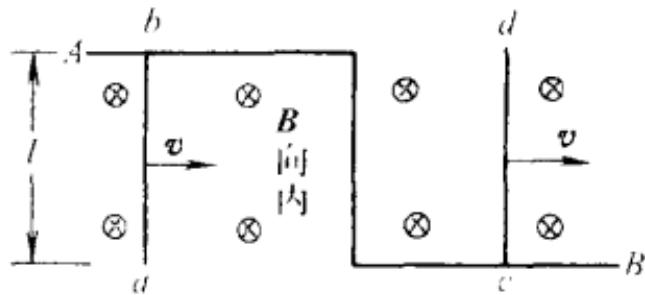
\includegraphics[width=0.5\linewidth]{figures/fig_8_1_23.jpg}
\end{center}

\vfill

\textbf{8.1.24.} 铁路的两条铁轨相距为 1435mm, 火车以每小时 100km 的速度前进, 火车所在处地磁场的磁感强度 B 在竖直方向上的分量为 0.15Gs. 两条铁轨除与车轮接通外, 彼此是绝缘的. 试求两条铁轨间的电势差 U.

$$
\mathrm{U} = B _ {\perp} l v = 0. 1 5 \times 1 0 ^ {- 4} \times 1 4 3 5 \times 1 0 ^ {- 3} \times \frac {1 0 0 \times 1 0 ^ {3}}{6 0 \times 6 0} = 6. 0 \times 1 0 ^ {- 4} (\mathrm{V})
$$

\vfill

\newpage

\textbf{8.1.25.} 飞机以 $v=200m/s$ 的速度水平飞行, 机翼两端相距 30m, 两端之间可当作连续导体. 已知飞机所在处地磁场的磁感强度 B 在竖直方向上的分量为 0.20Gs. 试求机翼两端的电势差 U.

$$
\text {   【解】   } U = B _ {\perp} l v = 0. 2 0 \times 1 0 ^ {- 4} \times 3 0 \times 2 0 0 = 0. 1 2 (\mathrm{V})
$$

\vfill

\textbf{8.1.26.} 一导体杆弯折成 N 形, 其中平行的两段长为 l. 当这导体杆以匀速 v 在磁感强度为 B 的均匀磁场中运动时, 设 B 与导体杆构成的平面垂直并向外, v 与 B 垂直, v 也与导体杆平行的两段垂直, 如图 8.1.26 所示. 试求导体杆两端 a、d 间的电势差 $U_{ad}$ .

\vfill

\newpage

\textbf{8.1.27.} 一段直导线长为 $l = 20\mathrm{cm}$ , 在中点 $b$ 折成 $\alpha = 30^{\circ}$ 角, 如图 8.1.27 所示. 磁场的磁感强度 $\pmb{B}$ 与这导线的两段都垂直. 这导线以速度 $\pmb{v}$ 运动, $\pmb{v}$ 的方向与 $ab$ 段一致, $v = 2.0\mathrm{m/s}$ , $B = 2.5 \times 10^{2}\mathrm{Gs}$ . 试求 $a, c$ 两端的电势差 $U_{ac}$ , 哪端电势高?

\vfill

\textbf{8.1.28.} 一根直导线 ab，在磁感强度为 B 的均匀磁场中以速度 v 平行移动，如图 8.1.28 所示。设 $r = ab$ ，试证明 a、b 两端的电势差为 $U_{ab} = B \times v \cdot r$ 。

\vfill

\newpage

\textbf{8.1.29.} 长为 l 的一段直导线在磁感强度为 B 的均匀磁场中以速度 v 运动，v 和 B 都与导线垂直，v 与 B 的夹角为 $\theta$ ，如图 8.1.29 所示。(1) 试求导线两端 a、b 的电势差 $U_{ab}$ ; (2) 当 $l = 60 ~cm, v = 5.0 ~m/s, B = 2.4 \times 10^{-2} ~T, \theta = 30^{\circ} ~时$ ，试计算 $U_{ab}$ 的值.

\vfill

\textbf{8.1.30.} 一条导线弯成半径为 $R$ 的半圆弧 $acb$ , 放在磁感强度为 $\pmb{B}$ 的均匀磁场中, $\pmb{B}$ 与半圆面垂直并向内, 如图 8.1.30(1)所示. 当它以速度 $\pmb{v}$ ( $\pmb{v}$ 与 $\pmb{B}$ 垂直, 并与 $ab$ 方向成 $45^{\circ}$ 角)运动时, 试求: (1) 这段导线中的感应电动势 $\mathcal{E}$ ; (2) 导线两端 $a, b$ 的电势差 $U_{ab}$ ; (3) 导线中点 $c$ 与 $b$ 端的电势差 $U_{cb}$ .

\vfill

\newpage

\textbf{8.1.31.} 载有电流 $I$ 的无穷长直导线旁边，有一段半径为 $R$ 的半圆形导线，圆心 $O$ 到 $I$ 的距离为 $l (> R)$ ，半圆形导线和电流 $I$ 在同一平面内，它的两端 $a, b$ 的联线与 $I$ 垂直，如图8.1.31所示。当它以匀速 $\pmb{v}$ 平行于电流 $I$ 运动时，试求它两端 $a, b$ 的电势差 $U_{ab}$

\vfill

\textbf{8.1.32.} 一无穷长直导线载有电流 I，在它旁边有一段直导线 AB, AB 与 I 垂直，并且在同一平面内，以速度 v 平行于 I 运动，如图 8.1.32 所示。已知 I = 10A, v = 5.0m/s, a = 1.0cm, b = 20.0cm。(1) 试求这段导线中的感应电动势 $\varepsilon$ ; (2) 导线 A、B 两端哪端电势高？(3) 如果用另一根导线把 A、B 两端联接起来，试问是否有电流流动？

\vfill

\newpage

\textbf{8.1.33.} 无穷长直线载有 $I = 5.0\mathrm{A}$ 的电流，旁边有一个与它共面的矩形线圈，长边与 $I$ 平行，长为 $l = 20\mathrm{cm}$ ，两边到 $I$ 的距离分别为 $a = 10\mathrm{cm}, b = 20\mathrm{cm}$ ，如图8.1.33所示。线圈共有 $N = 1000$ 币，以 $v = 3.0\mathrm{m / s}$ 的速度离开直导线。试求线圈里的感应电动势 $\mathcal{E}$ 。

图8.1.33
\begin{center}
    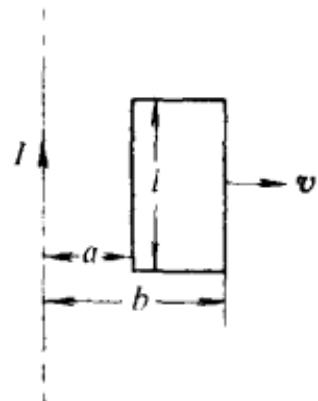
\includegraphics[width=0.5\linewidth]{figures/fig_8_1_33.jpg}
\end{center}

\vfill

\textbf{8.1.34.} 一条直导线横扫过磁感强度为 B 的磁场, B 在一圆柱空间内是均匀的, 在外面为零, 圆柱面的半径为 R, 如图 8.1.34(1) 所示. 当导线离圆柱轴线为 r 时, 导线的速度为 v, v 与导线垂直. 试求这时导线中产生的感应电动势 $\varepsilon$ .

\vfill

\newpage

\textbf{8.1.35.} 一矩形导线回路 abcd 处在磁感强度为 B 的均匀磁场中, B 与回路平面垂直并向外, 如图 8.1.35 所示. ab 边长为 l, 当它以速度 v 向右滑动时, 试求 a、b 两点的电势差 $U_{ab} = U_{a} - U_{b}$ . 哪点电势高?

\vfill

\textbf{8.1.36.} 两平行导线相距为 $l = 50\mathrm{cm}$ , 通过电阻 $R = 0.20\Omega$ 联接在一起, 放在磁感强度为 $\pmb{B}$ 的均匀磁场中, $\pmb{B}$ 与导线平面垂直并向内, 如图8.1.36所示, $B = 0.50\mathrm{T}$ ; 另一条导线 $ab$ 横跨在两平行导线上, 以匀速 $\pmb{v}$ 向右滑动, $\pmb{v}$ 与两导线平行, $v = 4.0\mathrm{m/s}$ . 试求: (1) 导线 $ab$ 的运动在闭合回路中所产生的感应电动势; (2) 电阻 $R$ 所消耗的功率 $P$ ; (3) 磁场 $\pmb{B}$ 作用在导线 $ab$ 上的力 $\pmb{F}$ .

\vfill

\newpage

\textbf{8.1.37.} 一横日字形导线框,如图 8.1.37(1)所示,已知 $ab = bc = cd = de = ef = fa = 0.10\mathrm{m}, ab, fc$ 和 $ed$ 各段电阻均为 $3.0\Omega, cd$ 和 $fe$ 两段电阻均为 $1.5\Omega$ , 而 $bc$ 和 $af$ 两段电阻均为零. 这导线框处在磁感强度为 $\pmb{B}$ 的均匀磁场中, $\pmb{B}$ 的方向与框面垂直并向内, $\pmb{B}$ 的大小为 $1.0\mathrm{T}$ ; 磁场的边界与 $de$ 边平行, 如图中虚线所示. 今以匀速 $\pmb{v}$ 将导线框从磁场中拉出, $\pmb{v}$ 与 $de$ 边垂直, $v = 2.4\mathrm{m/s}$ . 试求拉出导线框的力所作的功.

图8.1.37(1)

图8.1.37(2)
\begin{center}
    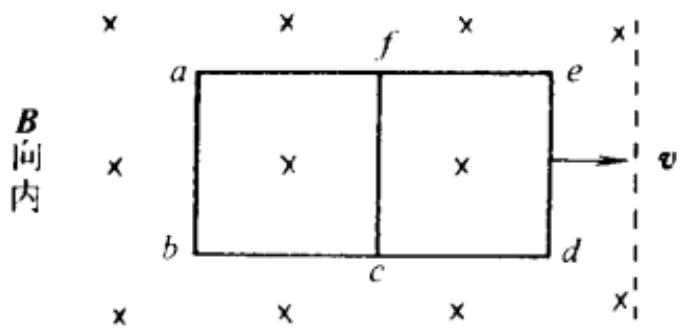
\includegraphics[width=0.5\linewidth]{figures/fig_8_1_37_1.jpg}
\end{center}
\begin{center}
    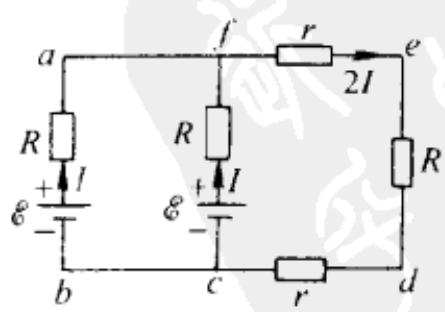
\includegraphics[width=0.5\linewidth]{figures/fig_8_1_37_2.jpg}
\end{center}

\vfill

\textbf{8.1.38.} 一矩形导线回路两边相距为 $l$ ，另一边 $ab$ 以匀速 $\pmb{v}$ 向右滑动， $\pmb{v}$ 与两边平行；整个回路都在磁感强度为 $\pmb{B}$ 的均匀磁场中， $\pmb{B}$ 与回路平面垂直并向外，如图8.1.38所示。 $\pmb{B}$ 随时间作如下变化： $B = B_0\cos \omega t$ 。试求 $ab$ 到左边的距离为 $x$ 时，回路中的感应电动势 $\varepsilon$ 。

图8.1.38
\begin{center}
    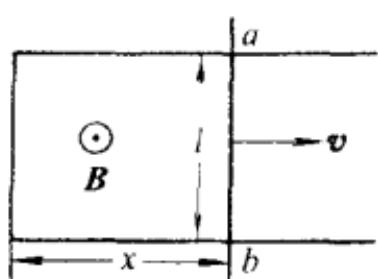
\includegraphics[width=0.5\linewidth]{figures/fig_8_1_38.jpg}
\end{center}

\vfill

\newpage

\textbf{8.1.39.} 两根竖直的金属杆相距为 $l$ ，上端通过电动势为 $\varepsilon$ 、内阻为 $r$ 的电池联接在一起，如图8.1.39所示。一质量为 $m$ 、电阻为 $R$ 的均质导体棒，两端分别套在两杆上，用手扶住让它静止。在空间有均匀磁场，磁感强度 $\pmb{B}$ 与杆棒构成的平面垂直。现放手让导体棒下落。设棒与杆间的摩擦力和杆本身的电阻都可略去不计，且杆足够长。试求棒下落的最大速度。

\vfill

\textbf{8.1.40.} 半径分别为 R 和 r 的两个大小圆线圈共轴, 中心相距为 x, 大线圈载有电流 I, 如图 8.1.40 所示. 设 $x \gg R$ , 大线圈中的电流 I 在小线圈处所产生的磁场可当作均匀磁场. 当小线圈以速度 v 沿轴线平行移动时, 试求小线圈内的感应电动势.

\vfill

\newpage

\textbf{8.1.41.} 一根金属杆, 上端 $a$ 有一小孔, 套在固定的水平轴上, 杆可以在磁场中来回摆动, 磁场的磁感强度 $\pmb{B}$ 与摆动平面垂直并向内, 如图 8.1.41 所示. 试问什么时候杆下端 $b$ 的电势高于上端 $a$ 的电势?

【解答】 $b, a$ 两端的电势差为

$$
\begin{array}{r l} U _ {b} - U _ {a} & = \int_ {b} ^ {a} \boldsymbol {E} _ {s} \cdot \mathrm{d} \boldsymbol {l} = \int_ {b} ^ {a} (- \boldsymbol {E} _ {i}) \cdot \mathrm{d} \boldsymbol {l} \\ & = \int_ {a} ^ {b} \boldsymbol {E} _ {i} \cdot \mathrm{d} \boldsymbol {l} = \int_ {a} ^ {b} \boldsymbol {v} \times \boldsymbol {B} \cdot \mathrm{d} \boldsymbol {l} \end{array}
$$

由上式可见，当 $v \times B$ 与 $ab$ 的方向相同时， $U_{b} - U_{a} > 0$ ，这时由图8.1.41可见，杆应向左摆动。即杆向左摆时，它下端的电势比上端的高。

图8.1.41

图8.1.42
\begin{center}
    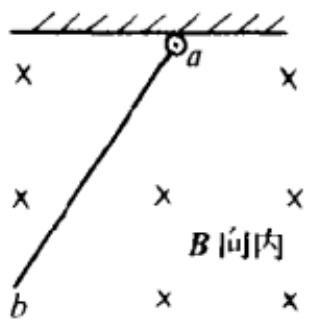
\includegraphics[width=0.5\linewidth]{figures/fig_8_1_41_1.jpg}
\end{center}
\begin{center}
    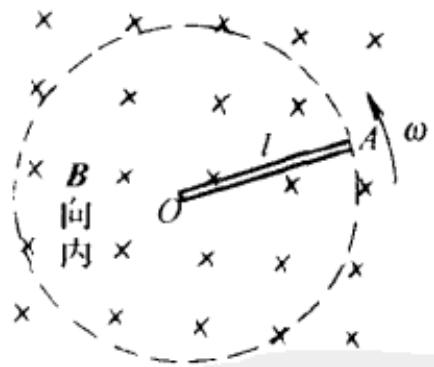
\includegraphics[width=0.5\linewidth]{figures/fig_8_1_41_2.jpg}
\end{center}

\vfill

\textbf{8.1.42.} 长为 l 的一根铜棒，在均匀磁场中以匀角速度 $\omega$ 转动，磁场的磁感强度 B 与棒垂直，转轴通过棒的一端并与 B 平行，如图 8.1.42 所示。(1)试求铜棒两端的电势差 $U_{OA}$ ，哪端电势高？(2)当 $l = 50 ~cm, B = 100 ~Gs$ ，转速为每秒 50 圈时，试计算 $U_{OA}$ 的值.

\vfill

\newpage

\textbf{8.1.43.} 只有一根辐条的轮子在均匀磁场中转动, 转动轴与磁感强度 B 平行, 如图 8.1.43 所示. 轮子和辐条都是导体, 辐条长为 R, 轮子每秒转 N 圈. 两条导线 a 和 b 通过各自的刷子分别与轮轴和轮缘接触. (1) 试求 a、b 间的感应电动势 $\varepsilon$ ; (2) 若在 a、b 间接一个电阻, 使辐条中的电流为 I, 试问 I 的方向如何? (3) 试求这时磁场作用在辐条上的力矩 M; (4) 当轮子反转时, I 是否也会反向?

图8.1.43

$$
\begin{array}{r l} \mathcal {E} & = \int_ {0} ^ {R} \boldsymbol {E} _ {i} \cdot \mathrm{d} \boldsymbol {l} = \int_ {0} ^ {R} \boldsymbol {v} \times \boldsymbol {B} \cdot \mathrm{d} \boldsymbol {l} = \int_ {0} ^ {R} v B \mathrm{d} l \\ & = \int_ {0} ^ {R} \omega l B \mathrm{d} l = \frac {1}{2} B \omega R ^ {2} = \frac {1}{2} B \cdot 2 \pi N \cdot R ^ {2} = N \pi B R ^ {2} \end{array} \tag {1}
$$

(2)电流 I 沿辐条向外.

(3)以 $e_{\omega}$ 为转动角速度 $\omega$ 方向上的单位矢量,如图8.1.43,其方向与B相同,则有

所以

$$
\begin{array}{l} \mathrm{d} \boldsymbol {M} = \boldsymbol {r} \times \mathrm{d} \boldsymbol {F} = \boldsymbol {r} \times (I \mathrm{d} l \times \boldsymbol {B}) = \boldsymbol {r} \times (I \mathrm{d} r \times \boldsymbol {B}) = - I B r \mathrm{d} r e _ {\omega} \\ \boldsymbol {M} = - I B \int_ {0} ^ {R} r \mathrm{d} r e _ {\omega} = - \frac {1}{2} I B R ^ {2} e _ {\omega} \end{array}
$$

负号表明,力矩 M 阻止轮子转动.

(4)电流 I 会反向.

\vfill

\textbf{8.1.44.} 半径为 R 的金属圆盘, 放在磁感强度为 B 的均匀磁场中, B 与盘面法线 n 的夹角为 $\theta$ , 如图 8.1.44 所示. 当这圆盘以每秒 N 圈的转速绕它的几何轴旋转时, 试求盘中心与边缘的电势差.
\begin{center}
    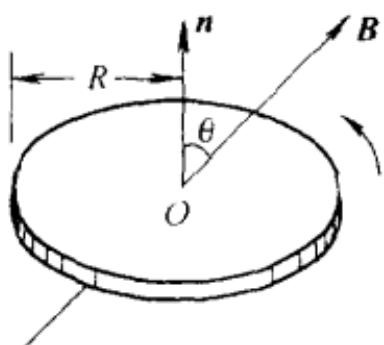
\includegraphics[width=0.5\linewidth]{figures/fig_8_1_44.jpg}
\end{center}

\vfill

\newpage

\textbf{8.1.45.} 由金属制成的直角三角形框架, 勾 BC 长为 a, 放在磁感强度为 B 的均匀磁场中, 股 AB 与 B 平行, 如图 8.1.45(1) 所示. 当这框架以股 AB 为轴, 每秒旋转 n 圈时, 试求勾 BC 里产生的感应电动势 $\varepsilon_{BC}$ 和整个框里产生的感应电动势 $\varepsilon$ .

\vfill

\textbf{8.1.46.} 一根 $50\mathrm{cm}$ 长的金属棒 $ab$ 水平放置，以长度的 $\frac{1}{5}$ 处为轴心，在水平面内旋转，每秒转两圈；已知该处地磁场的磁感强度 $\pmb{B}$ 在竖直方向上的分量 $B_{\perp} = 0.50$ 高斯，如图8.1.46(1)所示.试求棒两端的电势差 $U_{ab}$


图8.1.46(1)
图8.1.46(2)
\begin{center}
    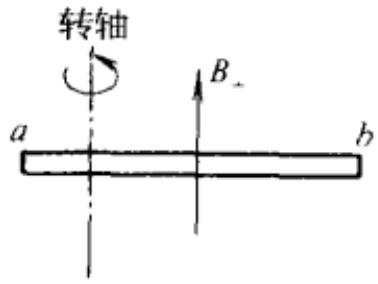
\includegraphics[width=0.5\linewidth]{figures/fig_8_1_46_1.jpg}
\end{center}
\begin{center}
    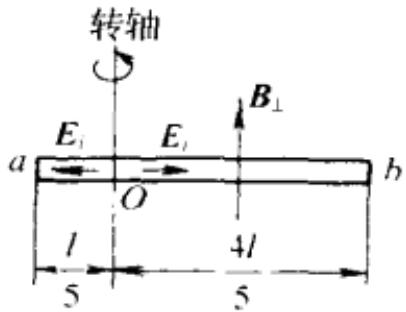
\includegraphics[width=0.5\linewidth]{figures/fig_8_1_46_2.jpg}
\end{center}

\vfill

\newpage

\textbf{8.1.47.} 横截面很小的金属丝弯成一圆环, 半径为 $a$ , 以角速度 $\omega$ 绕它的一个固定直径 $AB$ 旋转; 在它的中心, 有一个磁矩为 $m$ 的小磁棒, 其长度比 $a$ 小很多, $m$ 与 $\omega$ 同方向, 如图 8.1.47(1)所示, $C$ 为 $A, B$ 间的中点. (1)试求 $A, C$ 之间的感应电动势 $\varepsilon$ ; (2)怎样测量这个电动势?

\vfill

\textbf{8.1.48.} 一正方形线圈每边长 $100\mathrm{mm}$ , 在地磁场中转动, 每秒转 30 圈, 转轴通过中心并与一边平行. (1) 试问转轴与地磁场的磁感强度 $\pmb{B}$ 的夹角为什么值时, 线圈中产生的感应电动最大? (2) 设线圈所在处地磁的 $B = 0.55\mathrm{Gs}$ , 这时要在线圈中产生有效值为 $10\mathrm{mV}$ 的感应电动势, 试求线圈的匝数 $N$ .

\vfill

\newpage

\textbf{8.1.49.} 横截面积为 $1.0 ~mm^{2}$ 的铜线，弯成直径为 $a = 20 ~cm$ 的圆环，环面与地面垂直，该处地磁 B 的水平分量 $B_{\parallel} = 0.18 ~G s$ ，如图 8.1.49 所示。已知铜的电阻率为 $\rho = 1.75 \times 10^{-8} \Omega \cdot m$ 。当这圆环以每分钟 300 圈的匀角速度绕它的竖直直径转动时，试求：(1) 每秒产生的焦耳热；(2) 外加转矩的最大值。

\vfill

\textbf{8.1.50.} 最简单的交流发电机是在均匀磁场中转动的线圈, 转轴 $OO'$ 与磁场的磁感强度 B 垂直, 如图 8.1.50 所示. 已知 B = 8400Gs, 线圈面积 $S = 25cm^{2}$ , 线圈匝数 N = 20, 每秒转 50 圈. 设开始时线圈平面的法线与 B 垂直. 试求线圈中的电动势 $\varepsilon$ .

\vfill

\newpage

\textbf{8.1.51.} 法拉第圆盘发电机是一个在磁场中转动的导体圆盘. 设圆盘的半径为 $R$ , 转动轴线与它的几何轴重合, 磁感强度 $\pmb{B}$ 平行于轴线, 转动的角速度为 $\omega$ , 如图 8.1.51 所示. (1) 试求盘的边缘与中心的电势差 $U_{RO}$ , 并计算 $R = 15\mathrm{cm}, B = 0.60\mathrm{T}$ , 转速为每秒 30 圈时 $U_{RO}$ 的值; (2) 当盘反转时, 边缘与中心电势的高低是否也会倒过来?

\vfill

\textbf{8.1.52.} 一外表绝缘的导线,扭成如图 8.1.52 所示的三个圆形的平面闭合回路,它们的半径分别为 a、b、c, a > b > c. 这回路中都有磁感强度为 B 的均匀磁

场, 且 B 与回路的平面垂直并向内, 而回路外则无磁场. 当 B 的大小以速率 $\dot{B}$ 增大时, 试求回路中的感应电动势 $\varepsilon$ , 并指出中间圆 b 里感应电流的方向.

\vfill

\newpage

\textbf{8.1.53.} 用细导线做成一个半径为 $a$ 的圆环, 其电阻为 $R$ ; 另一根长为 $2a$ 的导线, 两端分别接在环上 $P, Q$ 两点, $\widehat{PQ}$ 为四分之一圆周, 导线折成直角, 中点 $O$ 在圆心, 如图 8.1.53(1) 所示. 这环内有磁感强度为 $B$ 的均匀磁场, 且 $B$ 与圆面垂直并向内, 而环外则无磁场. 当 $B$ 的大小以速率 $\dot{B}$ 增大时, 试求导线 $PO$ 中的电流.

\vfill

\textbf{8.1.54.} 一很长的直导线载有交流电流 $I = I_0 \sin \omega t$ ，它旁边有一长方形线圈ABCD，长为 $l$ ，宽为 $b - a$ ，线圈和导线在同一平面内，其长边与导线平行，如图8.1.54所示。试求：(1)穿过回路ABCD的磁通量 $\Phi$ ；(2)回路ABCD中的感应电动势 $\varepsilon$ 。

$$
\begin{array}{r l} & {\text {【解】}} \\ & {(1) \Phi = \int_ {a} ^ {b} B l \mathrm{d} r = \int_ {a} ^ {b} \frac {\mu_ {0} I _ {l}}{2 \pi r} l \mathrm{d} r = \frac {\mu_ {0} I _ {0} l \sin \omega t}{2 \pi} \int_ {a} ^ {b} \frac {\mathrm{d} r}{r} = \frac {\mu_ {0} I _ {0} l}{2 \pi} \left(\ln \frac {b}{a}\right) \sin \omega t} \\ & {(2) \varepsilon = - \frac {\mathrm{d} \Phi}{\mathrm{d} t} = - \frac {\mu_ {0} I _ {0} \omega l}{2 \pi} \left(\ln \frac {b}{a}\right) \cos \omega t} \end{array}
$$

\vfill

\newpage

\textbf{8.1.55.} 两条很长的平行输电线, 相距为 $l$ , 载有大小相等而方向相反的电流 $I = I_0 \cos \omega t$ ; 旁边有一长为 $a$ 、宽为 $b$ 的矩形线圈, 它们在同一平面内, 长边与输电线平行, 到最近一条的距离为 $d$ , 如图 8.1.55 所示. 试求线圈中的感应电动势 $\varepsilon$ .

\vfill

\textbf{8.1.56.} 一横截面积为 $S = 20\mathrm{cm}^2$ 的空心螺绕环，每厘米上绕有50匝线圈；环外绕有 $N = 5$ 匝的副线圈，副线圈与电流计G串联，构成一个电阻为 $r = 2.0\Omega$ 的闭合回路，如图8.1.56所示.今改变 $R$ 使螺绕环中的电流 $i$ 每秒减少20A.试求副线圈中的感应电动势 $\varepsilon$ 和感应电流 $I$

\vfill

\newpage

\textbf{8.1.57.} 一电子计算机里的存储元件是用矩磁材料(磁滞回线接近矩形的铁氧体)作成的小圆环,横截面积为 $0.15 \times 0.30 \mathrm{~mm}^2$ , 如图8.1.57(1)所示. 回路1中的电流 $I$ 使圆环由原来的剩磁状态 $B_r$ 翻转到另一剩磁状态 $-B_r[$ 图8.1.57(2)]. 已知 $B_r = 0.17 \mathrm{T}$ , 翻时间为 $\Delta t = 0.45 \mu \mathrm{s}$ . 试求回路2中感生电动势的大小.

\vfill

\textbf{8.1.58.} 一闭合线圈共有 N 匝,电阻为 R.试证明:当通过这线圈的磁通量改变 $\Delta\Phi$ 时,线圈内流过的电荷量为 $\Delta q=\frac{N\Delta\Phi}{R}$ .

\vfill

\newpage

\textbf{8.1.59.} 图 8.1.59 是测量螺线管内磁场的一种装置. 将一个很小的线圈放在

图8.1.59

待测处, 这线圈与测量电荷量的冲击电流计 G 串联. 当用反向开关 K 使螺线管的电流反向时, 测量线圈中就产生感应电动势, 从而产生电荷量 $\Delta q$ 的迁移; 由 G 测出 $\Delta q$ , 就可以算出测量线圈所在处磁感强度的大小 B 来. 已知测量线圈有 2000 匝, 它的直径为 2.5cm, 它和 G 串联回路的电阻为 1000Ω, 在 K 反向时测得 $\Delta q = 2.5 \times 10^{-7}$ 库仑. 试求被测处 B 的值.
\begin{center}
    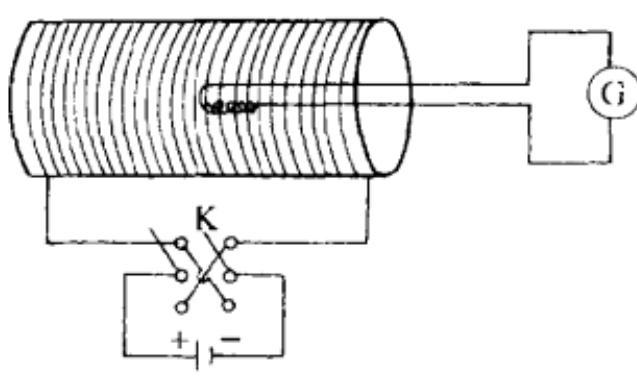
\includegraphics[width=0.5\linewidth]{figures/fig_8_1_59.jpg}
\end{center}

\vfill

\textbf{8.1.60.} 横截面直径为 $d$ 的无限长直螺线管，单位长度的匝数为 $n$ ，当它的导线中的电流按 $I = kt$ （ $k$ 为常数）的规律增大时，试求下列三处感应电场强度的大小：(1)管内轴线上；(2)管内离轴线为 $r$ 处；(3)管外离轴线为 $R$ 处.

\vfill

\newpage

\textbf{8.1.61.} 在圆柱形空间里有磁感强度为 B 的均匀磁场, B 平行于圆柱轴线, B 的大小 B 随时间 t 的变化关系为 $B = B_{0} - kt$ , 式中 $B_{0}$ 和 k 都是常量. 在这磁场里, 有一条长为 l 的直导线 ab, 位于圆柱的横截面内, 到圆柱轴线的距离为 h, 如图 8.1.61(1) 所示. 试求这段导线里的感生电动势.

\vfill

\textbf{8.1.62.} 一圆柱形空间内有磁感强度为 B 的均匀磁场，其横截面的半径为 R, B 平行于轴线向外，如图 8.1.62(1) 所示。在这横截面内有一条长为 l 的直导线，其两端 a、b 在圆柱面上。当 B 的大小以速率 $\dot{B}$ 增大时，试求导线两端的电势差 $U_{ab}$ 。

\vfill

\newpage

\textbf{8.1.63.} 在半径为 $R$ 的圆柱形空间里有磁感强度为 $\pmb{B}$ 的均匀磁场， $\pmb{B}$ 与圆柱的轴线平行， $\pmb{B}$ 的大小随时间 $t$ 变化的规律为 $B = B_0 + kt$ ，式中 $B_0$ 和 $k$ 都是常量；圆柱外的空间里磁感强度为零。有一条长为 $2R$ 的直导线 $ab$ 在圆柱的横截面内，它的一端 $a$ 和中点 $c$ 都在圆柱面上，如图8.1.63(1)所示。试求这导线两端的电势差 $U_{ab}$ 。

图8.1.63(1)

图8.1.63(2)
\begin{center}
    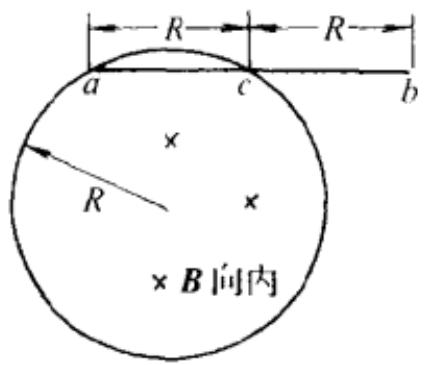
\includegraphics[width=0.5\linewidth]{figures/fig_8_1_63_1.jpg}
\end{center}
\begin{center}
    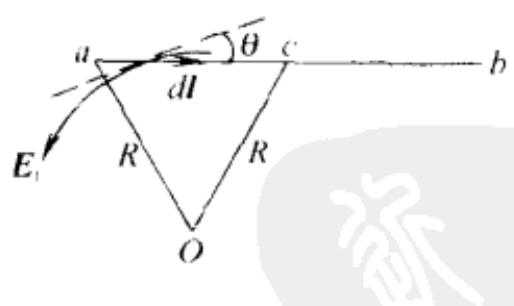
\includegraphics[width=0.5\linewidth]{figures/fig_8_1_63_2.jpg}
\end{center}

\vfill

\textbf{8.1.64.} 一半径为 $a$ 的无限长直圆筒均匀带电，电荷量的面密度为 $\sigma$ ，从 $t = 0$ 时刻由静止开始，以匀角加速度 $\alpha$ 绕它的几何轴旋转.试求 $t$ 时刻下列三处的感应电场强度：(1)轴线上的 $\pmb{E}_0$ ;(2)筒内离轴线为 $r$ 处的 $\pmb{E}_r$ ;(3)筒外离轴线为 $R$ 处的 $\pmb{E}_R$

\vfill

\newpage

\textbf{8.1.65.} 半径为 r 的金属圆环, 由两个半圆弧联接而成, 一半 $aR_{1}b$ 的电阻为 $R_{1}$ , 另一半 $aR_{2}b$ 的电阻为 $R_{2}$ ; 这圆环放在有均匀磁场的圆柱形空间里, 它们的几何轴重合, 磁感强度 B 与几何轴平行并向内, 如图 8.1.65(1) 所示. (1) 设 B 的大小 B 以 $\frac{dB}{dt} = k (>0)$ 增大时, 试求 a、b 两点的电势差 $U_{ab} = U_{a} - U_{b}$ ; (2) 导体内的感应电动势的方向 (即涡旋电场 $E_{i}$ 的方向) 是否总是由低电势指向高电势?

图8.1.65(1)
\begin{center}
    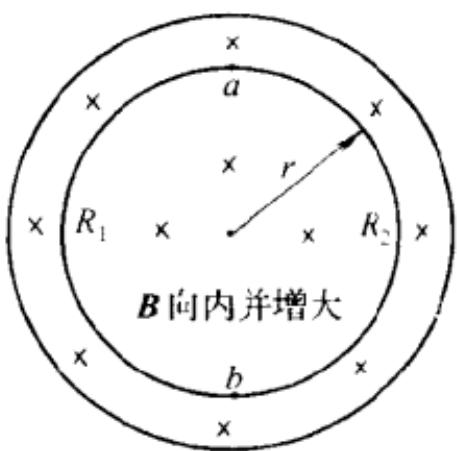
\includegraphics[width=0.5\linewidth]{figures/fig_8_1_65.jpg}
\end{center}

\vfill

\textbf{8.1.66.} 如图 8.1.66, 一铜片可以绕 $OO'$ 轴摆动, 摆动时扫过磁场, 磁场的磁感强度 $\pmb{B}$ 与铜片表面垂直。(1) 如果铜片扫过磁场的部分是像图上那样的长齿, 则铜片的摆动同没有磁场时差不多, 要来回摆动很多次才逐渐停止; (2) 如果铜片上扫过磁场的部分不是长齿, 而是整片, 则铜片的摆动很快就会停止下来. 这种现象在仪表中常用来使运动的部件(如指针)很快停止下来. 为什么铜片的形状对摆动有影响? 试说明其道理.

【解答】整块铜片在磁场中摆动时，因切割磁力线而产生感应电流(涡流)，磁场作用在这电流上的力阻止铜片运动，所以铜片很快就会停止下来。如果铜片扫过磁场的部分是像图8.1.66那样的长齿，则齿槽阻止了涡流的形成，所以磁场阻止铜片运动的力就很小，因而铜片要摆动很多次才能停止下来。

\vfill

\newpage

\textbf{8.1.67.} 汽车上有一种转速表,如图 8.1.67 所示,其中永磁铁与汽车发动机的转轴相连,当汽车行驶时,永磁铁被带动旋转;磁铁的旋转使它上面的铝盘 A 受到力矩的作用而发生偏转,铝盘的轴上装有弹簧 S 和指针 P. 当铝盘所受的力矩与弹簧的反力矩平衡时,铝盘便偏转在某个位置,这时指针 P 就指出车速的值.试说明铝盘转动的道理.

【解答】铝盘与永磁铁有相对运动时，铝盘切割磁力线产生感应电流，感应电流受永磁铁的磁场作用力(安培力)使铝盘跟随永磁铁转动.
\begin{center}
    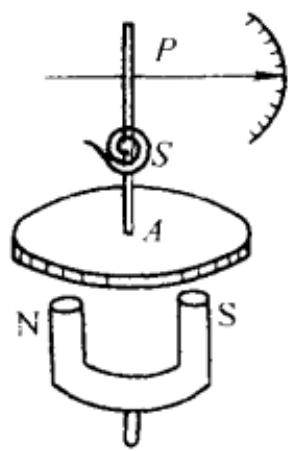
\includegraphics[width=0.5\linewidth]{figures/fig_8_1_67.jpg}
\end{center}

\vfill

\textbf{8.1.68.} 鼠笼式感应电动机是小功率(如几千瓦)交流电动机中最常用的一种.它的转子是在两个铜(或铝)环上,安装

图8.1.67

一些铜(或铝)条而成,形如鼠笼,可以绕它的几何轴 $OO'$ 转动,如图8.1.68(1)(a)所示.在使用时,电源来的电并不通过转子,而是通过转子外面的定子(线圈),定子中的电流在转子所在处产生一个旋转磁场,这磁场的方向与转子的轴线 $OO'$ 垂直,并且绕着 $OO'$ 旋转,如图8.1.68(1)(b)所示.在这种磁场的作用下,转子便会跟随磁场转动.试说明:(1)转子转动的道理;(2)转子的转速恒小于磁场的转速.

(a)

(b)
图8.1.68(1)

【解答】（1）如图8.1.68(2)(a)，设 $\pmb{B}$ 正向纸面内旋转，这等于 $\pmb{B}$ 不动，铜(或铝)条向外运动所产生的效果。这时感应电动势的非静电力 $E_{i} = \pmb{v} \times \pmb{B}$ 使铜条内的感应电流 $I$ 沿 $E_{i}$ 的方向流动。磁场 $\pmb{B}$ 作用在这电流上的安培力 $\mathrm{dF} = I\mathrm{d}l \times \pmb{B}$ 其方向如图8.1.68(2)(b)所示，垂直于纸面向内，即 $\mathrm{dF}$ 的方向是向着 $\pmb{B}$ 旋转的方向。因此，转子受这安培力的作用，便跟着磁场转动。

(a)

(b)
图8.1.68(2)

(2) 只有转子的转速小于磁场的转速时, 铜条才能切割磁力线, 这时才有使转子转动的安培力. 若转子的转速达到磁场的转速, 便没有使转子转动的安培力, 这时轴上的摩擦力便会使转子减速. 因此, 转子的转速恒小于磁场的转速.
\begin{center}
    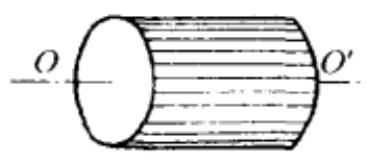
\includegraphics[width=0.5\linewidth]{figures/fig_8_1_68_1.jpg}
\end{center}
\begin{center}
    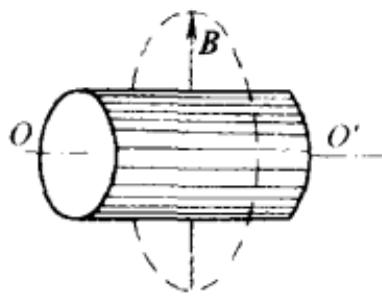
\includegraphics[width=0.5\linewidth]{figures/fig_8_1_68_2.jpg}
\end{center}
\begin{center}
    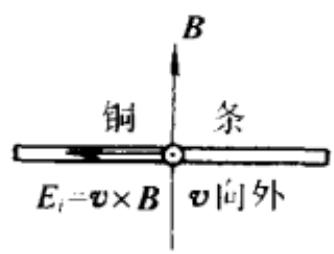
\includegraphics[width=0.5\linewidth]{figures/fig_8_1_68_3.jpg}
\end{center}
\begin{center}
    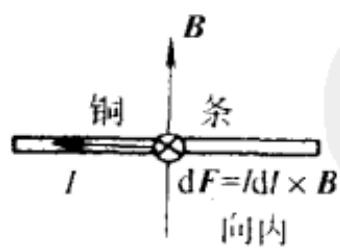
\includegraphics[width=0.5\linewidth]{figures/fig_8_1_68_4.jpg}
\end{center}

\vfill

\newpage

\textbf{8.1.69.} 在竖立的铁心上绕有线圈,在它上面放一个铝环,如图 8.1.69 所示.当把线圈的两头 a 和 b 接到适当的交流电源上时,铝环便立刻跳将起来.(1)试说明铝环为什么会跳起来;(2)如果让线圈持续接通交流电源,铝环将会怎样?并说明原因.

【解答】（1）铝环电阻非常小，它里面的感应电流很大，感应电流与线圈中的电流的相位差接近 $\pi$ ，在一个周期，这两个电流的方向几乎总是相反的，因而铝环所受的安培力对一个周期的平均值是相当大的排斥力(向上的力).当这力超过铝环的重量时，铝环便跳起.

(2)这时铝环便悬浮在线圈上的一定高度处.因为铝环离线圈越远,它所受的安培力就越小.当铝环在某一高度处,安培力与重力达到平衡,铝环便悬浮在那里.这是一个很容易演示的实验.

图8.1.69

图8.1.70
\begin{center}
    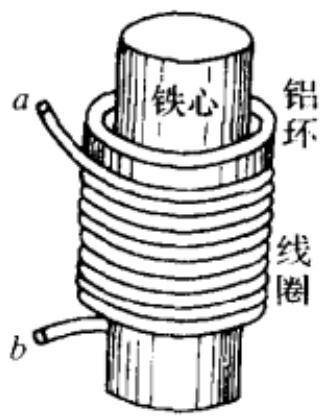
\includegraphics[width=0.5\linewidth]{figures/fig_8_1_69_1.jpg}
\end{center}
\begin{center}
    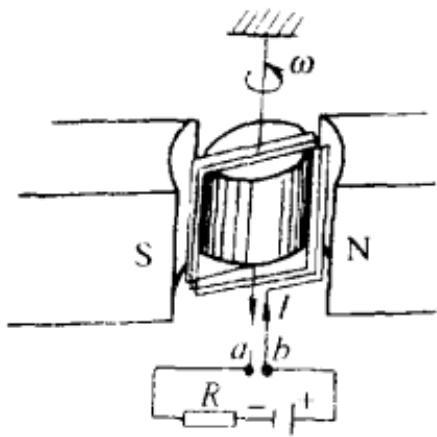
\includegraphics[width=0.5\linewidth]{figures/fig_8_1_69_2.jpg}
\end{center}

\vfill

\textbf{8.1.70.} 灵敏电流计由悬挂在永磁场(磁感强度为 B)中的线圈构成,如图8.1.70所示.线圈的面积为 S,匝数为 N,电阻为 $R_{g}$ . 将电流通入线圈时,线圈便以悬丝为轴转动,转动惯量为 J,悬丝的扭转常数为 D,线圈以外的电阻为 R.(1)试列出线圈运动的微分方程;(2)试求线圈停止时偏转的角度(以通过线圈的电流 I=0 时,线圈停止的位置为零点);(3)线圈到达偏转角最快而不振荡称为中肯状态,试求使电流计处于中肯状态的条件.

\vfill

\newpage

\textbf{8.1.71.} 灵敏电流计在回到零点时,一般都要振荡很久才能停下来.为了防止这种现象发生,可在电流计的两个接头上接上一个阻尼电键,当灵敏电流计回到零点时,接通这个电键,它便立刻停下来.试说明其道理.

【解答】阻尼电链接通,灵敏电流计的线圈被短路,电阻立刻由无穷大变到最小,感应电流就立刻由零增加到很大,它受到磁场作用的安培力(阻力)就很大,因而电流计就立刻停下来.

\vfill

\textbf{8.1.72.} 灵敏电流计在回到零点时,一般都要振荡很久才能停下来.为了防止这种现象发生,可在电流计的线圈上套一个由较粗导线构成的闭合线圈(阻尼线圈),这样,它就不再振荡了.试说明其道理.

【解答】阻尼线圈由于电阻很小,当它随电流计的线圈在磁场中转动时,因切割磁力线而产生很大的感应电流,这电流受磁场的作用力(安培力)就很大,它阻止线圈运动,所以电流计就不振荡了.

\vfill

\newpage

\textbf{8.1.73.} 利用变化的磁场所产生的感应电场来加速电子的装置叫做电子感应加速器, 它的结构如图 8.1.73 所示. 由交变电流 I 激励的电磁铁产生强磁场 B, B 的变化所产生的感应电场(涡旋电场)用来加速电子, 同时 B 本身又维持电子在环形真空室内运动. 试分析在简谐交流电 I 的一个周期里, 哪一个时间可用来加速电子.


(2) 环形真空室俯视图
图8.1.73
\begin{center}
    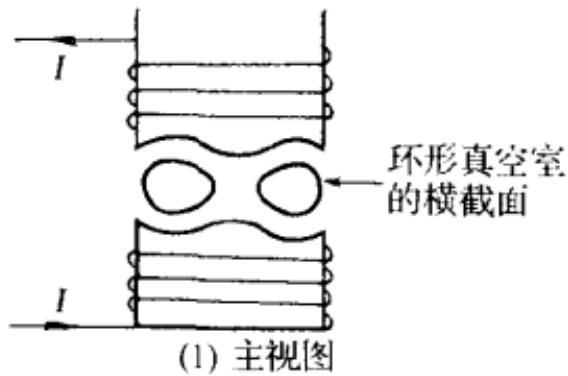
\includegraphics[width=0.5\linewidth]{figures/fig_8_1_73_1.jpg}
\end{center}
\begin{center}
    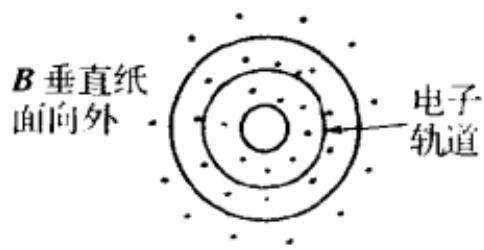
\includegraphics[width=0.5\linewidth]{figures/fig_8_1_73_2.jpg}
\end{center}

\vfill

\textbf{8.1.74.} 在一电子感应加速器中,电子加速的时间是 4.2ms. 电子轨道内磁通量的最大值为 1.8Wb.(1)试求电子沿轨道加速时,平均每绕行一圈所获得的能量;(2)设电子开始时速度为零,最后的动能为 100MeV,试问它共绕行了多少圈?(3)若轨道半径为 84cm,试问它在加速过程中共走了多少路程?

\vfill

\newpage

\textbf{8.1.75.} 电子感应加速器是利用变化的磁场 B 所产生的感应电场(涡旋电场) $E_{i}$ 来加速电子, 同时 B 本身又维持电子在固定的圆轨道上运动, 如图 8.1.75 所

示. 设开始时, $B = 0$ , 电子的初速为零; 加速后, 电子轨道处磁感强度 $\pmb{B}$ 的大小为 $B$ , 电子轨道内的平均磁感强度的大小为 $\overline{B} = \int \pmb{B} \cdot d\pmb{S} / \pi R^2$ (式中 $R$ 为电子轨道半径), 则当 $B = \frac{1}{2} \overline{B}$ 时, 电子便可在半径为 $R$ 的固定圆轨道上加速运动. 试证明上述结论.

图8.1.75
\begin{center}
    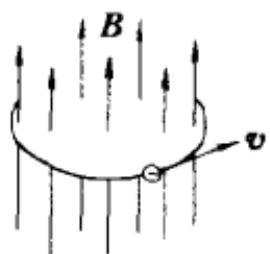
\includegraphics[width=0.5\linewidth]{figures/fig_8_1_75.jpg}
\end{center}

\vfill

\textbf{8.2.1.} 将磁棒插入闭合线圈时, 线圈里便会产生感应电流. 以线圈为参考系 $S$ , 磁棒为参考系 $S'$ . 相对于 $S$ 系静止的观测者看来, 线圈不动而磁棒动, 磁场发生了变化, 产生了感应电场 $\pmb{E}_i$ , 从而引起感应电流. 相对于 $S'$ 系静止的观测者看来, 磁棒不动而线圈在磁棒的磁场里运动, 它里面的自由电子因受到洛伦兹力 $f = -ev \times B$ 而产生定向运动, 从而形成感应电流. 可见对于线圈里产生感应电流这同一现象, 相对于 $S$ 系静止的观测者和相对于 $S'$ 静止的观测者的看法是不同的. (1) 你认为上述两种看法哪个对? (2) 对同一现象有两种不同的看法, 这意味着什么?

【解答】（1）相对于 S 系静止的观测者来说，磁场变化产生感应电流的看法是对的；相对于 $S'$ 系静止的观测者来说，在磁场中运动的线圈内自由电子因受洛伦兹力而产生感应电流的看法是对的.

(2)这意味着, $E_{i}$ 和 $v\times B$ 之间有某种关系. 这种关系就是狭义相对论得出的电磁场的变换关系.
\begin{center}
    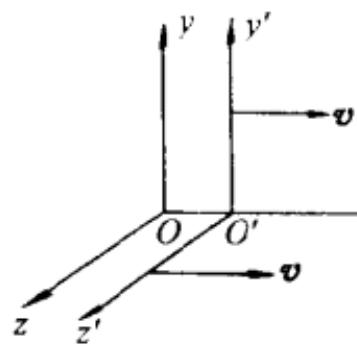
\includegraphics[width=0.5\linewidth]{figures/fig_8_2_1.jpg}
\end{center}

\vfill

\newpage

\textbf{8.2.2.} 设 $S'(x', y', z')$ 系以匀速 $\pmb{v} = (v, 0, 0)$ 相对于 $S(x, y, z)$ 系运动，如图8.2.2所示。一电磁场的电场强度和磁感强度在 $S(x, y, z)$ 系里测量分别为 $\overrightarrow{x}, x'\mathbf{E} = (E_x, E_y, E_z), \mathbf{B}(B_x, B_y, B_z)$ ；在 $S'(x', y', z')$ 系里测量分别为 $\mathbf{E}' = (E_x', E_y', E_z'), \mathbf{B}' = (B_x', B_y', B_z')$ 。根据狭义相对论，它们之间的变换关系为

图8.2.2

$$
\begin{array}{r l} E _ {x} ^ {\prime} = E _ {x}, & E _ {y} ^ {\prime} = \gamma (E _ {y} - v B _ {z}), \\ E _ {z} ^ {\prime} = \gamma (E _ {z} + v B _ {y}) \\ B _ {x} ^ {\prime} = B _ {x}, & B _ {y} ^ {\prime} = \gamma (B _ {y} + \frac {v}{c ^ {2}} E _ {z}), \\ B _ {z} ^ {\prime} = \gamma (B _ {z} - \frac {v}{c ^ {2}} E _ {y}) \end{array}
$$

式中 $\gamma = \frac{1}{\sqrt{1 - \frac{v^2}{c^2}}}, c$ 为真空中的光速. 试求这个变换的逆变换.

\vfill

\textbf{8.2.3.} 在惯性系 $S(x, y, z)$ 内有均匀磁场，其磁感强度为 $\pmb{B} = (0, 0, B)$ ；另一参考系 $S'(x', y', z')$ 以匀速 $\pmb{v} = (v, 0, 0)$ 相对于 $S(x, y, z)$ 系运动，如图8.2.3所示。试求在 $S'(x', y', z')$ 系观测到的电磁场 $E'$ 和 $B'$ 。

\vfill

\newpage

\textbf{8.2.4.} 在惯性坐标系 $S(x, y, z)$ 中，有一不随时间变化的均匀磁场 $\pmb{B} = (0, 0, B)$ . 在这磁场中，有一静长为 $l_0$ 的金属杆 $ab$ 平行于 $y$ 轴，并以匀速 $\pmb{v} = (v, 0, 0)$ 相对于 $S(x, y, z)$ 系运动，如图8.2.4所示。(1)试求杆两端的电势差 $U_{ab}$ ; (2)在跟随杆运动的坐标系 $S'(x', y', z')$ 中，试求杆两端的电势差 $U_{ab}'$ ; (3) $U_{ab}'$ 与 $U_{ab}$ 相等吗？

图8.2.4 【解】（1）在感应电场 $\pmb{E}_i = \pmb{v} \times \pmb{B}$ 的作用下，金属杆上出现电荷，这电荷产生静电场 $\pmb{E}_s$ 。平衡时， $\pmb{E}_s = -\pmb{E}_i$ 。故得杆两端的电势差为

$$
\begin{array}{r l} U _ {a t} & = U _ {a} - U _ {b} = \int_ {a} ^ {b} \boldsymbol {E} _ {s} \cdot \mathrm{d} \boldsymbol {l} \\ & = \int_ {a} ^ {b} (- \boldsymbol {E} _ {i}) \cdot \mathrm{d} \boldsymbol {l} \\ & = - \int_ {a} ^ {b} \boldsymbol {v} \times \boldsymbol {B} \cdot \mathrm{d} \boldsymbol {l} \\ & = - v B l _ {0} \end{array}\tag{1}
$$

式中负号表示 a 端电势比 b 端低.

(2) 根据狭义相对论的电磁场变换关系[参见前面8.2.2题], $S'(x', y', z')$ 系的电场强度 $\pmb{E}'$ 的分量为

$$
E _ {x} ^ {\prime} = E _ {x} = 0\tag{2}
$$

$$
E _ {y} ^ {\prime} = \gamma (E _ {y} - v B _ {z}) = - \gamma v B\tag{3}
$$

$$
E _ {z} ^ {\prime} = \gamma (E _ {z} + v B _ {y}) = \gamma (0 + 0) = 0\tag{4}
$$

式中

$$
\gamma = \frac {1}{\sqrt {1 - \frac {v ^ {2}}{c ^ {2}}}}\tag{5}
$$

于是得 $a, b$ 两端的电势差为

$$
U _ {a b} ^ {\prime} = U _ {a} ^ {\prime} - U _ {b} ^ {\prime} = \int_ {a} ^ {b} \boldsymbol {E} _ {s} ^ {\prime} \cdot \mathrm{d} l ^ {\prime} = \int_ {a} ^ {b} (- \gamma v B) \mathrm{d} l _ {y} ^ {\prime} = - \gamma v B l _ {0}\tag{6}
$$

(3)严格说来， $U_{ab}^{\prime}\neq U_{ab}$ .但实际上，由于 $v\ll c$ ，故在测量误差范围内， $U_{ab}^{\prime}=U_{ab}$

\vfill

\textbf{8.2.5.} 在惯性坐标系 $S(x, y, z)$ 中，有一不随时间变化的磁场 $\pmb{B} = (0, 0, B)$ . 在这磁场中，有一静长为 $l_0$ 的金属杆 $ab$ 位于 $x - y$ 平面内，与 $x$ 轴的夹角为 $30^\circ$ ，以匀速 $\pmb{v} = (v, 0, 0)$ 相对于 $S(x, y, z)$ 系运动，如图8.2.5所示.(1)试求杆两端的电势差 $U_{ab}$ ;(2)根据狭义相对论的电磁场变换关系，试求跟随杆运动的坐标系 $S'$

图8.2.5

$(x', y', z')$ 中的电场强度 $E'$ ，并由 $E'$ 求杆两端的电势差 $U_{ab}'$ .
\begin{center}
    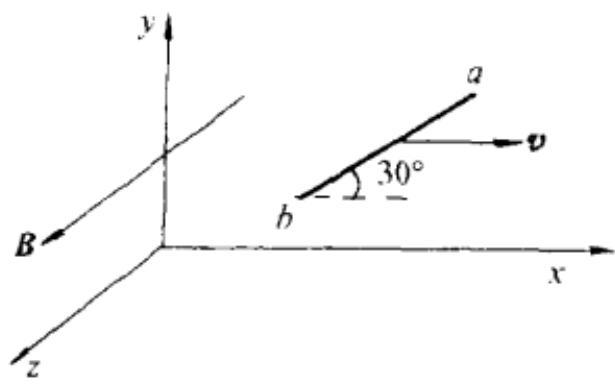
\includegraphics[width=0.5\linewidth]{figures/fig_8_2_5.jpg}
\end{center}

\vfill

\newpage

\textbf{8.2.6.} 一无穷长直导线载有稳定电流 $I$ ，一飞机正以匀速 $v$ 飞离这导线，机翼两端 $a, b$ 相距为 $l, ab$ 与导线平行，到导线的距离为 $r$ ，如图8.2.6(1)所示。(1)试求在飞机上观测，电流 $I$ 所产生的电场强度 $E'$ 以及机翼两端的电势差 $U_{ab}'$ ；(2)若飞机的飞行方向反过来，如图8.2.6(2)所示，这时在飞机上观测到的电场强度和机翼两端的

电势差各如何？

\vfill

\textbf{8.2.7.} 一无穷长直导线载有电流 $I$ ，另一段直导线 $AB$ 与电流 $I$ 共面，并与 $I$ 垂直， $A, B$ 两端到 $I$ 的距离分别为 $a$ 和 $b$ ，这段导线以匀速 $\pmb{v}$ 平行于电流 $I$ 运动，如图8.2.7所示。（1）试求导线两端的电势差 $U_{AB}$ ；（2）在跟随导线 $AB$ 运动的坐标系里，试求电流 $I$ 所产生的电场强度和导线两端的电势差 $U_{AB}'$ ；（3）当 $I = 5.0\mathrm{A}, a = 1.0\mathrm{m}, b = 2.0\mathrm{m}, v = 1.0\mathrm{m/s}$ 时，试求上述两种电势差的值。

图8.2.7
\begin{center}
    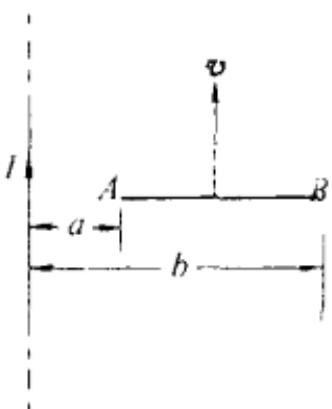
\includegraphics[width=0.5\linewidth]{figures/fig_8_2_7.jpg}
\end{center}

\vfill

\newpage

\textbf{8.2.8.} 一无穷长直导线载有电流 $I = 5.0\mathrm{A}$ , 旁边有一个与它共面的矩形线圈, 长边与导线平行, 如图8.2.8所示. 线圈共有 $N = 1000$ 匝, 以匀速 $v = 3.0\mathrm{m / s}$ 离开导线. 已知 $a = 10\mathrm{cm}, l = b = 20\mathrm{cm}$ . (1)试求线圈里的感应电动势 $\mathcal{E}$ ; (2)以线圈为参照系 $S'$ , 试求导线中的电流 $I$ 在 $S'$ 系里产生的电场 $E'$ , 从而由 $E'$ 求线圈中的电动势 $\mathcal{E}'$ .

$$
\begin{array}{r l} \mathcal {E} & = N \oint \boldsymbol {E} _ {i} \cdot \mathrm{d} \boldsymbol {l} = N \oint \boldsymbol {v} \times \boldsymbol {B} \cdot \mathrm{d} \boldsymbol {l} \\ & = N v B _ {a} l - N v B _ {b} l = N v l \frac {\mu_ {0} I}{2 \pi} (\frac {1}{a} - \frac {1}{b}) \\ & = 1 0 0 0 \times 3. 0 \times 2 0 \times 1 0 ^ {- 2} \end{array}
$$

$$
\begin{array}{r l} & \times \frac {4 \pi \times 1 0 ^ {- 7} \times 5 . 0}{2 \pi} \times (\frac {1 0 0}{1 0} - \frac {1 0 0}{2 0}) \\ & = 3. 0 \times 1 0 ^ {- 3} (\mathrm{V}) \end{array}\tag{1}
$$

(2)在相对于导线静止的参考系(S)中,电磁场为

$$
\boldsymbol {E} = 0, \quad \boldsymbol {B} = \frac {\mu_ {0} I}{2 \pi r} \boldsymbol {e}\tag{2}
$$

式中 e 为电流 I 的右手螺旋方向上的单位矢量. 在相对于线圈静止的参考系 $(S')$ 中, 根据狭义相对论的电磁场变换关系[参见前 8.2.7 题的式(2)], 电场强度为

$$
\boldsymbol {E} _ {\parallel} ^ {\prime} = \boldsymbol {E} _ {\parallel} = 0, \quad \boldsymbol {E} _ {\perp} ^ {\prime} = \gamma (\boldsymbol {E} _ {\perp} + \boldsymbol {v} \times \boldsymbol {B}) = \gamma \boldsymbol {v} \times \boldsymbol {B}\tag{3}
$$

于是得所求的电动势为

$$
\begin{array}{r l} \mathcal {E} ^ {\prime} & = \oint \gamma \boldsymbol {v} \times \boldsymbol {B} \cdot \mathrm{d} \boldsymbol {l} = \oint \gamma v \frac {\mu_ {0} N I}{2 \pi r} \mathrm{d} r \\ & = \gamma N v l \frac {\mu_ {0} I}{2 \pi} (\frac {1}{a} - \frac {1}{b}) = \gamma \mathcal {E} \\ & = \frac {1}{\sqrt {1 - \left(\frac {3 . 0}{3 \times 1 0 ^ {8}}\right) ^ {2}}} \times 3. 0 \times 1 0 ^ {- 3} = 3. 0 \times 1 0 ^ {- 3} (\mathrm{V}) \end{array}\tag{4}
$$

\vfill

\textbf{8.2.9.} 一磁偶极矩为 $p_{m}$ 的小磁棒产生的磁场为

$$
\begin{array}{c} B _ {r} = \frac {p _ {\mathrm{m}} \cos \theta}{2 \pi r ^ {3}} \\ B _ {\theta} = \frac {p _ {\mathrm{m}} \sin \theta}{4 \pi r ^ {3}} \end{array}
$$

图8.2.9(1)

离小磁棒为 $b$ 处有一半径为 $a$ 的导线圈，其轴线与小磁棒重合，以匀速 $\pmb{v}$ 沿轴线运动，如图8.2.9(1)所示.(1)试求导线圈中的感应电动势 $\mathcal{E}$ ；(2)在相对于导线圈静止的坐标系 $S'$ 中，试求小磁棒所产生的电场强度 $\pmb{E}'$ ，并由 $\pmb{E}'$ 求导线圈中的感应电动势 $\mathcal{E}'$ .

图 8.2.9(2)
\begin{center}
    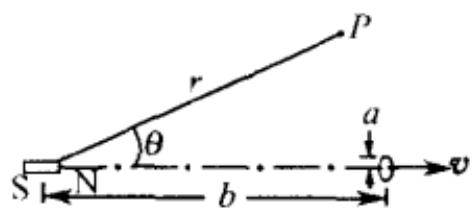
\includegraphics[width=0.5\linewidth]{figures/fig_8_2_9_1.jpg}
\end{center}
\begin{center}
    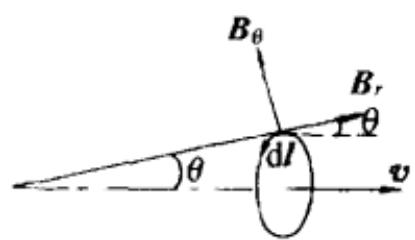
\includegraphics[width=0.5\linewidth]{figures/fig_8_2_9_2.jpg}
\end{center}

\vfill

\newpage

\textbf{8.3.1.} 一个自感为 $L$ 的线圈接在电路中, 电流 $I$ 自 $a$ 端流入, 从 $b$ 端流出, 如图 8.3.1(1) 所示. 由于有自感电动势 $\varepsilon_{L} = -L \frac{\mathrm{d} I}{\mathrm{d} t}$ , 故 $L$ 便是一个电动势为 $\varepsilon_{L}$ 的电源. 试问这个电源的正极是 $a$ 还是 $b$ ?

【解答】电流 I 流入处 a 为电源 $\varepsilon_{L}$ 的负极，流出处 b 为正极。说明如下。

图8.3.1(1)

图8.3.1(2)

图8.3.1(3)

如图8.3.1(2)，当 $I$ 减小时，感应电场 $\pmb{E}_i$ 与 $I$ 同方向，故 $a$ 为电源 $\varepsilon_{L}$ 的负极， $b$ 为正极。这

时 $\varepsilon_{L} = -L \frac{dI}{dt} > 0,$ 与实际情况符合.

如图8.3.1(3)，当 $I$ 增大时，感应电场 $\pmb{E}_i$ 与 $I$ 反方向。这时 $a$ 为电源 $\varepsilon_L$ 的正极， $b$ 为负极。好像与上面所说的“电流 $I$ 流入处 $a$ 为电源 $\varepsilon_L$ 的负极”刚好相反。可是，这时 $\varepsilon_L = -L\frac{\mathrm{d}l}{\mathrm{d}t} < 0$ 。一个电动势为负的电源，其正极就是电动势为正的电源的负极。所以，这时 $b$ 实际上就是负极。
\begin{center}
    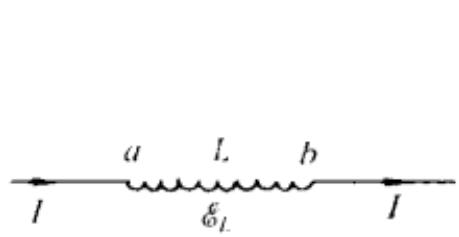
\includegraphics[width=0.5\linewidth]{figures/fig_8_3_1_1.jpg}
\end{center}
\begin{center}
    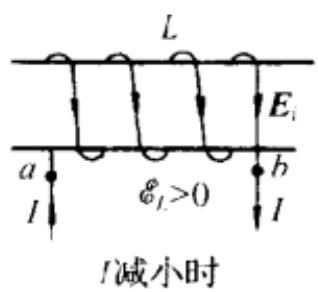
\includegraphics[width=0.5\linewidth]{figures/fig_8_3_1_2.jpg}
\end{center}
\begin{center}
    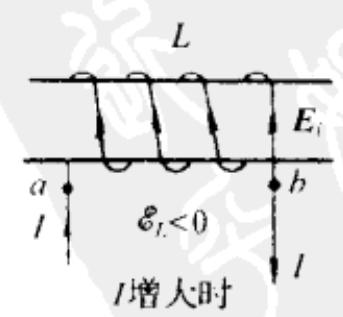
\includegraphics[width=0.5\linewidth]{figures/fig_8_3_1_3.jpg}
\end{center}

\vfill

\textbf{8.3.2.} 在长 60cm、直径为 5.0cm 的空心纸筒上绕多少匝线圈，才能得到自感为 $6.0 \times 10^{-3}H$ 的线圈？

\vfill

\newpage

\textbf{8.3.3.} 一纸筒长 $30\mathrm{cm}$ , 直径为 $3.0\mathrm{cm}$ , 上面绕有 500 匝线圈. (1) 试求这个线圈的自感 $L_{0}$ ; (2) 如果在这线圈内放入 $\mu_{\mathrm{r}} = 5000$ 的铁心, 试求这时的自感 $L$ .

$$
\begin{array}{r l} \text {【解】} & (1) L _ {0} = \mu_ {0} n ^ {2} V = \mu_ {0} (\frac {N}{l}) ^ {2} V = \mu_ {0} \frac {N ^ {2}}{l} S \\ & \qquad = 4 \pi \times 1 0 ^ {- 7} \times \frac {5 0 0 ^ {2}}{3 0 \times 1 0 ^ {- 2}} \times \pi \times \left(\frac {3 . 0 \times 1 0 ^ {- 2}}{2}\right) ^ {2} \\ & \qquad = 7. 4 \times 1 0 ^ {- 4} (\mathrm{H}) \\ (2) L = \mu_ {r} \mu_ {0} n ^ {2} V = \mu_ {r} L _ {0} = 5 0 0 0 \times 7. 4 \times 1 0 ^ {- 4} \\ & \qquad = 3. 7 (\mathrm{H}) \end{array}
$$

\vfill

\textbf{8.3.4.} 一螺线管由表面绝缘的细导线密绕而成，长为 $l$ ，横截面的半径为 $R$ ，单位长度的匝数为 $n$ ，管内充满磁导率为 $\mu$ 的均匀介质.已知 $R\ll l$ .试求这螺线管的自感 $L$

图8.3.4
\begin{center}
    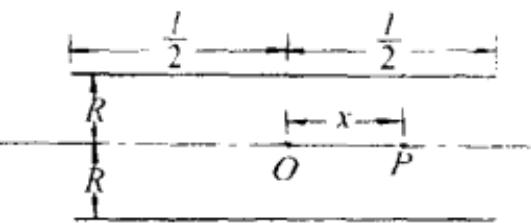
\includegraphics[width=0.5\linewidth]{figures/fig_8_3_4.jpg}
\end{center}

\vfill

\newpage

\textbf{8.3.5.} 在磁导率为 $\mu$ 的圆柱形磁介质上, 用表面绝缘的细导线绕两个线圈: 原线圈 $N_{1}$ 匝, 副线圈 $N_{2}$ 匝, 它们的长度都是 $l$ , 横截面积都是 $S$ , 如图 8.3.5 所示. 设 $\sqrt{S} \ll l$ , 略去边缘效应. 试求: (1) 两线圈各自的自感 $L_{1}$ 和 $L_{2}$ ; (2) 两线圈之间的互感 $M$ ; (3) $M$ 与 $L_{1}$ 和 $L_{2}$ 的关系.

图8.3.5
\begin{center}
    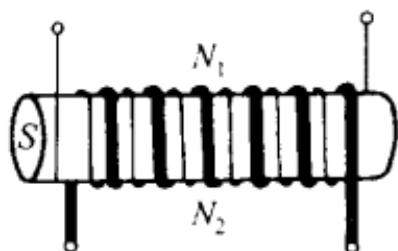
\includegraphics[width=0.5\linewidth]{figures/fig_8_3_5.jpg}
\end{center}

\vfill

\textbf{8.3.6.} 一螺线管长为 l，横截面积为 S，由 $N_{1}$ 匝表面绝缘的细导线密绕而成；在它的中部，绕有 $N_{2}$ 匝表面绝缘的导线，如图 8.3.6 所示。(1)试求这两线圈的互感 M；(2)当 $l = 1.00 \, m, S = 10 \, cm^{2}, N_{1} = 1000$ 匝， $N_{2} = 20$ 匝时，试计算 M 的值.

\vfill

\newpage

\textbf{8.3.7.} 两螺线管共轴, 长度都是 $l$ , 里面螺线管的半径为 $a_1$ , 匝数为 $N_1$ ; 外面螺线管的半径为 $a_2 (>a_1)$ , 匝数为 $N_2$ , 如图 8.3.7 所示. 略去边缘效应, 试求这两螺线管的自感与它们的互感之间的关系.

\vfill

\textbf{8.3.8.} 一螺线管长为 $l$ , 横截面积为 $S$ , 单位长度的匝数为 $n$ , 可以看成是两个长为 $\frac{l}{2}$ 的螺线管在中间串联而成, 如图 8.3.8 所示. 如按公式 $L = \mu_0 n^2 S l$ 计算, 则有

$$
L = \mu_ {0} n ^ {2} S (\frac {l}{2} + \frac {l}{2})
$$

$$
= L _ {1} + L _ {2}
$$

如按顺串联的公式计算,则为

$$
L = L _ {1} + L _ {2} + 2 M
$$

式中 M 是两个 $\frac{l}{2}$ 的螺线管之间的互感. 比较以上两式, 便会得出 M = 0 的结论.
(1)你认为这个结论是否正确？为什么？(2)问题出在哪里？

【解答】（1） $M = 0$ 的结论显然不正确，因长度都是 $\frac{l}{2}$ 的两个线圈彼此都有磁力线进入对方，故 $M \neq 0$ .

(2)问题出在, $L=\mu_{0}n^{2}Sl$ 不是准确公式,而是在 $\sqrt{S}\ll l$ 的条件下,略去边缘效应而得出的粗糙近似公式,比实际自感大一些[参见前面8.3.4题].因此,公式 $L=\mu_{0}n^{2}Sl$ 不适用于讨论上面的问题.如果用较好一些的近似公式[参见前面8.3.4题的式(8)] $L=\mu_{0}n^{2}Sl\left[\sqrt{1+(\frac{R}{l})^{2}-\frac{R}{l}}\right]$ (式中R为螺线管的半径),就不会得出M=0的结论了.

\vfill

\newpage

\textbf{8.3.9.} 有一种汽车点火线圈由绕在同一轴管上的两个彼此绝缘的线圈构成, 长为 $l = 10\mathrm{cm}$ , 半径为 $r = 3.0\mathrm{cm}$ , 其中一个有 $N_{1} = 16000$ 匝, 另一个有 $N_{2} = 400$ 匝, 如图 8.3.9 所示. 当原线圈中的电流在万分之一秒里改变 3.0A 时, 试求副线圈里的感应电动势. (这电动势在电花隙中产生火花, 以点燃汽油与空气的混合物.)

图8.3.9
\begin{center}
    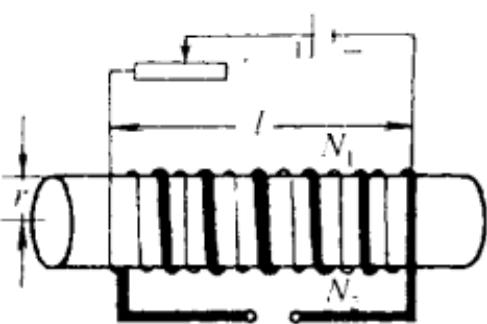
\includegraphics[width=0.5\linewidth]{figures/fig_8_3_9.jpg}
\end{center}

\vfill

\textbf{8.3.10.} 有的电阻是用电阻丝绕成的,为了减少自感,常用双绕法,如图 8.3.10 所示.试说明为什么这样绕自感就很小.

【解答】因为这样绕,反方向的电流其磁场互相削弱,故磁通量很小,所以自感 L 就很小. [参见后面 8.3.35 题(1)]

图8.3.10 8.3.11 一螺绕环中心线的长度为 $l$ ，横截面积为 $S$ ，由 $N$ 匝表面绝缘的导线密绕而成。设 $\sqrt{S} \ll l$ ，试求它的自感 $L$ ，并计算 $l = 1.0\mathrm{m}$ ， $S = 10\mathrm{cm}^2$ ， $N = 1000$ 匝时 $L$ 的值。

\vfill

\newpage

\textbf{8.3.12.} 一螺绕环由 N 匝表面绝缘的细导线在纸环上密绕而成, 横截面是长为 b-a、宽为 h 的矩形, 环的内外半径分别为 a 和 b, 它的一半如图 8.3.12 所示. 试求它的自感 L, 并计算当 N=1000 匝, a=5.0cm, b=10cm, h=1.0cm 时 L 的值.

\vfill

\textbf{8.3.13.} 一螺绕环横截面的半径为 $a$ ，中心线的半径为 $R, R \gg a$ ，它是由表面绝缘的导线密绕而成，共有两个线圈，一个 $N_1$ 匝，另一个 $N_2$ 匝。试求：(1)两线圈的自感 $L_1$ 和 $L_2$ ；(2)两线圈间的互感 $M$ ；(3) $M$ 与 $L_1$ 和 $L_2$ 的关系。

\vfill

\newpage

\textbf{8.3.14.} 一正方形铁环, 边长为 $l$ , 横截面积为 $S$ , 磁导率为 $\mu = \mu_{\mathrm{r}} \mu_{0}$ . 已知 $\sqrt{S} \ll l, \mu_{\mathrm{r}} \gg 1$ . 在它的一边用表面绝缘的导线绕有 $N$ 匝线圈, 如图 8.3.14 所示. 试求这线圈的自感 $L_{ab}$ .

\vfill

\textbf{8.3.15.} 一铁心长为 $l$ ，弯成方形，在一边留有宽为 $\delta$ 的空气间隙，铁心的横截面积为 $S$ ，磁导率为 $\mu = \mu_{\mathrm{r}} \mu_0$ ；在它的一边用表面绝缘的导线绕有 $N$ 匝线圈，如图8.3.15所示。已知 $\sqrt{S} \ll l, \mu_{\mathrm{r}} \gg 1$ 。试求线圈的自感 $L_{ab}$ ，并计算 $l = 56.5 \mathrm{~cm}, S =$

图8.3.15

$3.1\mathrm{cm}^2, \delta = 1.0\mathrm{mm}, \mu_{\mathrm{r}} = 500, N = 1000$ 匝时 $L_{ab}$ 的值.
\begin{center}
    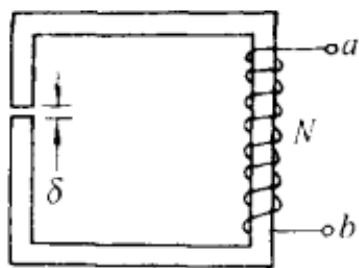
\includegraphics[width=0.5\linewidth]{figures/fig_8_3_15.jpg}
\end{center}

\vfill

\newpage

\textbf{8.3.16.} 一空心螺绕环的自感为 $L_{0}$ , 加入铁心后自感为 $L_{1}$ , 在铁心上锯开一个很窄的断口后自感为 $L_{2}$ . 试比较 $L_{0}, L_{1}, L_{2}$ 三者的大小.

\vfill

\textbf{8.3.17.} 一螺绕环由表面绝缘的细导线在磁导率为 $\mu$ 的铁环上密绕 $N$ 匝而成, 环的平均半径为 $R$ , 横面积为 $S, \sqrt{S} \ll R$ , 如图 8.3.17 所示. 这螺绕环可以看成是两个 $\frac{N}{2}$ 匝的半环形线圈 $ac$ 和 $cb$ 串联而成. 试求这两个半环形线圈 $ac$ 和 $cb$ 之间的互感.
\begin{center}
    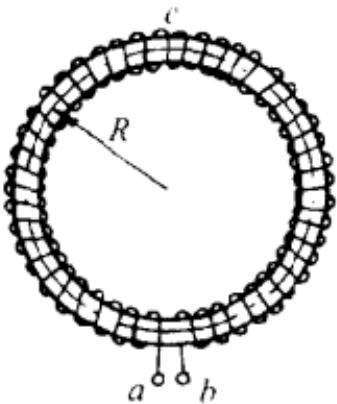
\includegraphics[width=0.5\linewidth]{figures/fig_8_3_17.jpg}
\end{center}

\vfill

\newpage

\textbf{8.3.18.} 一铁环的长度为 $l$ ，横截面积为 $S$ ，磁导率为 $\mu = \mu_{\mathrm{r}} \mu_0$ ，已知 $l \gg \sqrt{S}, \mu_{\mathrm{r}} \gg 1$ 。用表面绝缘的细导线在这铁环上绕两个线圈，一个为 $N_1$ 匝，另一个为 $N_2$ 匝，两线圈的长度相等，都是 $\frac{l}{4}$ ，如图8.3.18所示。试求这两个线圈的自感 $L_{ab}$ 和 $L_{cd}$ 以及它们之间的互感 $M$ 。

图8.3.18

\vfill

\textbf{8.3.19.} 一线圈的自感为 $L_{1}$ , 在它旁边有一个自感为 $L_{2}$ 、电阻可略去不计的线圈, 两线圈之间的互感为 $M$ , 如图 8.3.19 所示. 试证明: 如果把互感的作用也考虑在自感里, 则 $L_{1}$ 的有效自感为 $L_{1} - M^{2} / L_{2}$ .

\vfill

\newpage

\textbf{8.3.20.} 两个平面线圈的面积分别为 $S_{1}$ 和 $S_{2}$ , 所载电流分别为 $I_{1}$ 和 $I_{2}$ , 如图8.3.20所示. 设 $I_{1}$ 所产生的磁场通过 $S_{2}$ 的磁通量为 $\Phi_{21}, I_{2}$ 产生的磁场通过 $S_{1}$ 的磁通量为 $\Phi_{12}$ . 试问当 $S_{2} = 2S_{1}$ 和 $I_{2} = I_{1}$ 时, $\Phi_{21}$ 与 $\Phi_{12}$ 哪个大些?

图8.3.20

【解答】一样大，即 $\Phi_{21}=\Phi_{12}$

因 $\Phi_{21} = M_{21}I_1, \Phi_{12} = M_{12}I_2$ ，而 $M_{21} = M_{12}$ . 今 $I_2 = I_1$ ，故得 $\Phi_{21} = \Phi_{12}$ .
\begin{center}
    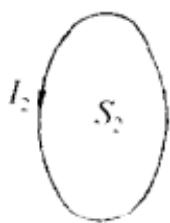
\includegraphics[width=0.5\linewidth]{figures/fig_8_3_20_1.jpg}
\end{center}
\begin{center}
    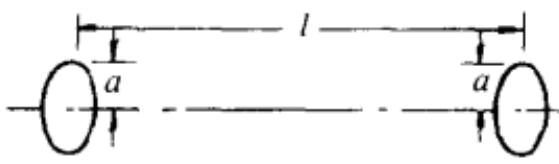
\includegraphics[width=0.5\linewidth]{figures/fig_8_3_20_2.jpg}
\end{center}

\vfill

\textbf{8.3.21.} 两个相同的圆线圈共轴, 它们的半径都是 a, 匝数都是 N, 中心相距为 l, 如图 8.3.21 所示. 已知 $a \ll l$ , 试求它们之间的互感.

图8.3.21 【解】设一个线圈的电流为 $I_{1}$ ，它在另一个线圈中心产生的磁感强度 $\pmb{B}_{21}$ 的大小为[参见前面5.1.20题的式(2)]

$$
B _ {2 1} = \frac {\mu_ {0} N I _ {1} a ^ {2}}{2 (l ^ {2} + a ^ {2}) ^ {3 / 2}}\tag{1}
$$

$B_{21}$ 的方向沿轴线. 因 $a \ll l$ , 故线圈内的 $B_{21}$ 可看作近似均匀磁场, 于是得通过线圈的磁链为

$$
\Psi_ {2 1} = N \Phi_ {2 1} = N B _ {2 1} \cdot \pi a ^ {2} = \frac {\pi \mu_ {0} N ^ {2} a ^ {4} I _ {1}}{2 (l ^ {2} + a ^ {2}) ^ {3 / 2}}\tag{2}
$$

由此得两线圈之间的互感为

$$
M = \frac {\Psi_ {2 1}}{I _ {1}} = \frac {\pi \mu_ {0} N ^ {2} a ^ {4}}{2 (l ^ {2} + a ^ {2}) ^ {3 / 2}}\tag{3}
$$
\begin{center}
    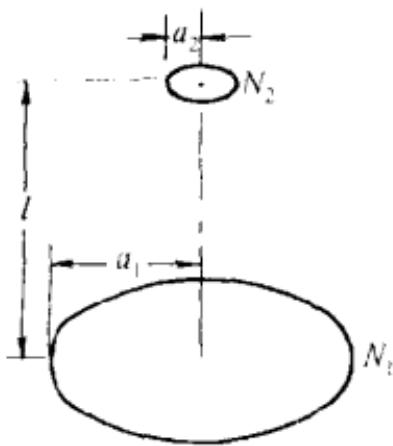
\includegraphics[width=0.5\linewidth]{figures/fig_8_3_21.jpg}
\end{center}

\vfill

\newpage

\textbf{8.3.22.} 共轴的两个圆线圈, 半径分别为 $a_1$ 和 $a_2$ , 匝数分别为 $N_1$ 和 $N_2$ , 圆心相距为 $l$ , 如图 8.3.22 所示. 设 $a_2 \ll a_1$ 和 $l$ , 试求它们之间的互感 $M$ .

\vfill

\textbf{8.3.23.} 一圆线圈由 n=50 匝表面绝缘的细导线绕成，圆面积为 $S=4.0cm^{2}$ ，放在另一个半径为 R=20cm 的大圆形线圈中心，两者共轴，如图 8.2.23 所示。已知大线圈由 N=100 匝表面绝缘的导线绕成。（1）试求这两线圈之间的互感 M；（2）当大线圈中的电流每秒减少 50A 时，试求小线圈中的感应电动势 $\varepsilon$ 。

图8.3.23
\begin{center}
    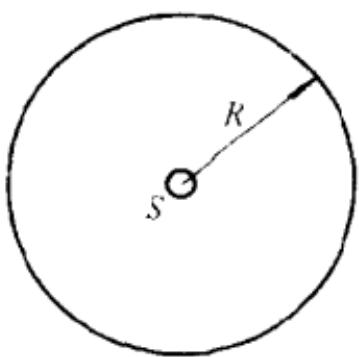
\includegraphics[width=0.5\linewidth]{figures/fig_8_3_23.jpg}
\end{center}

\vfill

\newpage

\textbf{8.3.24.} 半径为 $r$ ，匝数为 $n$ 的圆线圈，放在半径为 $R$ 、匝数为 $N$ 的大圆线圈中心，两线圈在同一平面内且轴线重合。（1）试证明：当 $R \gg r$ 时，这两线圈的互感近似为 $M = \pi \mu_0 n N r^2 / 2R$ ；（2）试用上面的结果证明：当磁矩为 $m$ 的小磁棒放在上述大线圈中心，两者轴线重合时，通过大线圈的磁链近似为 $\Psi = \mu_0 N m / 2R$ 。

\vfill

\textbf{8.3.25.} 一大圆线圈半径为 $a$ ，共有 $N$ 匝。一磁偶极矩为 $p_m$ 的小磁棒沿它的轴线抽出，在离中心为 $x$ 处时，抽出速度为 $\pmb{v}$ ，如图8.3.25所示。(1)试证明：这时在大线圈中产

图8.3.25

生的感应电动势的大小近似为 $\varepsilon=\frac{3Na^{2}p_{m}xv}{2(x^{2}+a^{2})^{3/2}}$ ; (2) 设大线圈是电阻为 R 的闭合线圈, 试证明: 当小磁棒从大线圈中心移到无穷远时, 大线圈中流过的电荷量近似为 $Q=\frac{Np_{m}}{2aR}$ .
\begin{center}
    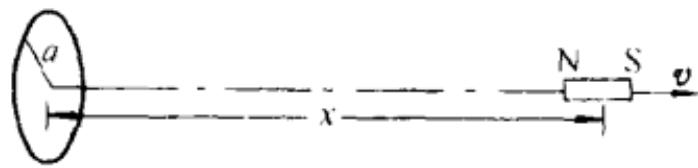
\includegraphics[width=0.5\linewidth]{figures/fig_8_3_25.jpg}
\end{center}

\vfill

\newpage

\textbf{8.3.26.} 一同轴电缆可看作是无限长的两个同轴导体圆筒, 内外筒的半径分别为 $R_{1}$ 和 $R_{2}$ , 电流沿内筒流去, 沿外筒流回, 电流都均匀分布在筒的横截面上. 两筒间充满磁导率为 $\mu$ 的介质. 试求这同轴电缆单位长度的自感.

\vfill

\textbf{8.3.27.} 一同轴传输线由很长的两个同轴导体薄圆筒构成,内筒半径为 $R_{1}=$

40mm, 外筒半径为 $R_{2}=120mm$ , 两筒间是空气. 在两筒间加上 U=10V 电压时, 电流由一筒流去, 由另一筒流回, 大小为 I=10mA, 电流在两筒上都是均匀分布的. a 是两筒间很靠近内筒的一点, b 是两筒间很靠近外筒的一点. 试求: (1)a、b 两点电场强度和电位移的值; (2)a、b 两点磁场强度和磁感强度的值; (3) 单位长度的电容; (4) 单位长度的自感.

\vfill

\newpage

\textbf{8.3.28.} 一同轴电缆由很长的直导线和套在它外面的同轴导体圆筒构成,导线的半径为 a, 圆筒的半径为 b, 它们之间介质的 $\mu_{r}=1$ . 使用时,电流沿导线流去,沿圆筒流回. 设电流在圆筒上和在导线的横截面上都是均匀分布的. 试求这电缆单位长度的自感.

\vfill

\textbf{8.3.29.} 两条平行长直导线, 横截面的半径都是 a, 中心相距为 d, 属于同一回路. 设两导线内部的磁通量都可略去不计, 试求这两导线单位长度的自感.

\vfill

\newpage

\textbf{8.3.30.} 两条平行的长直输电线,属于同一回路,电流方向相反,它们的半径分别为 a 和 b，轴线相距为 d，电流都均匀分布在它们各自的横截面上。试求它们单位长度的自感，并计算 $a = b = 10 \, mm, d = 20 \, cm$ 时单位长度自感的值。

\vfill

\textbf{8.3.31.} 一磁导率为 $\mu$ 的铁环, 内半径为 $a$ , 外半径为 $b$ , 横截面是高为 $h$ 的矩形, 在它上面用表面绝缘的导线绕有 $N$ 匝线圈, 如图 8.3.31 所示. 在这导线的几何轴上, 有一条无穷长直导线, 试求导线与线圈间的互感.

\vfill

\newpage

\textbf{8.3.32.} 一矩形线圈长为 $a = 20\mathrm{cm}$ , 宽为 $b = 10\mathrm{cm}$ , 由100匝表面绝缘的导线绕成, 放在一很长的直导线旁边, 且与该导线在同一平面内. 该导线是另一闭合回路的一部分, 其他部分离线圈都很远, 影响可略去不计. 试求图8.3.32中(1)和(2)两种情况下, 线圈与导线之间的互感.

图8.3.32

\vfill

\textbf{8.3.33.} 一无穷长直导线旁边有一与它共面的圆形线圈, 半径为 a, 圆心到导线的距离为 l, l > a, 如图 8.3.33(1) 所示. 试证明: 它们之间的互感为 $M = \mu_{0}(l -$

$$
\sqrt {l ^ {2} - a ^ {2}})
$$

图8.3.33(1)

图8.3.33(2)
\begin{center}
    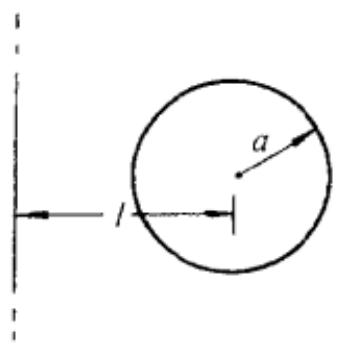
\includegraphics[width=0.5\linewidth]{figures/fig_8_3_33_1.jpg}
\end{center}
\begin{center}
    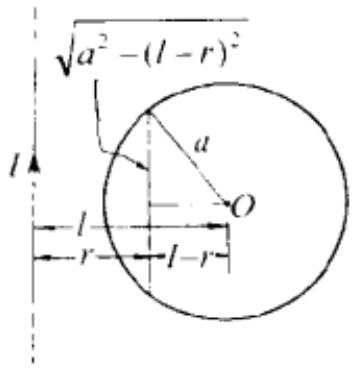
\includegraphics[width=0.5\linewidth]{figures/fig_8_3_33_2.jpg}
\end{center}

\vfill

\newpage

\textbf{8.3.34.} 一对相同的导体薄片,互相平行放置,长为 l,宽为 b,相距为 a,a≪b≪l,如图8.3.34所示.当这对导体片用作传输线时,电流沿片长方向流动,自一片流去,由另一片流回.设

图8.3.34

电流均匀分布在片的宽度上,略去边缘效应,试求它的自感 L.
\begin{center}
    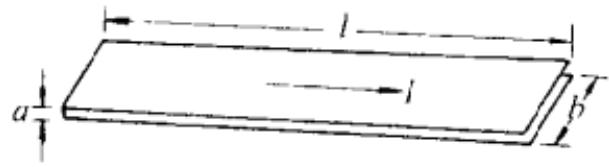
\includegraphics[width=0.5\linewidth]{figures/fig_8_3_34.jpg}
\end{center}

\vfill

\textbf{8.3.35.} 在一纸筒上绕有两个相同的线圈 $(a,b)$ 和 $(a',b')$ ，如图8.3.35所示，每个线圈的自感都是0.050H.试求：(1)a和 $a'$ 相接时，b和 $b'$ 间的自感；(2) $a'$ 和b相接时，a和 $b'$ 间的自感.

图8.3.35 【解】设两线圈都可当作是密绕的长螺线管，边缘效应可略去不计，则对其中一个线圈(长为 $l$ ，横截面积为 $S$ ，匝数为 $N$ )，当载有电流 $I$ 时，里面的磁感强度为

$$
B = \mu_ {0} \frac {N}{l} I\tag{1}
$$

磁链为

$$
\Psi = N \Phi = N B S = \mu_ {0} \frac {N ^ {2}}{l} S I\tag{2}
$$

其自感为

$$
L = \frac {\Psi}{I} = \mu_ {0} \frac {N ^ {2}}{l} S = 0. 0 5 0 H\tag{3}
$$

(1)这时两线圈中的电流大小相等而方向相反,故线圈内的 B=0, 因而磁链 $\Psi=0$ , 故所求的自感为

$$
L _ {b b ^ {\prime}} = \frac {\Psi}{I} = 0\tag{4}
$$

(2)这时两线圈中的电流大小相等而方向相同,因而自感等于匝数为 2N 的线圈的自感,即所求的自感为

$$
L _ {a b ^ {\prime}} = \mu_ {0} \frac {(2 N) ^ {2}}{l} S = 4 \mu_ {0} \frac {N ^ {2}}{l} S = 4 \times 0. 0 5 0 = 0. 2 0 (\mathrm{H})\tag{5}
$$

【别解】（1）因两线圈相同且绕在一起，故

$$
L _ {1} = L _ {2} = M = 0. 0 5 0 \mathrm{H}\tag{6}
$$

这时两线圈是反串联，故所求的自感为

$$
L _ {b b ^ {\prime}} = L _ {1} + L _ {2} - 2 M = 0\tag{7}
$$

(2)这时两线圈是顺串联,故所求的自感为

$$
L _ {a b ^ {\prime}} = L _ {1} + L _ {2} + 2 M = 4 L _ {1} = 4 \times 0. 0 5 0 = 0. 2 0 (\mathrm{H})\tag{8}
$$

\vfill

\newpage

\textbf{8.3.36.} 两线圈的自感分别为 $L_{1}$ 和 $L_{2}$ , 它们之间的互感可略去不计, 试求它们串联后的总自感 $L$ .

\vfill

\textbf{8.3.37.} 两线圈的自感分别为 $L_{1}$ 和 $L_{2}$ , 它们之间的互感为 $M$ , 试求下列两种情况下它们串联后的总自感: (1) 顺串联, 如图8.3.37(1), 1和4之间的自感; (2) 反串联, 如图8.3.37(2), 1和3之间的自感.

\vfill

\newpage

\textbf{8.3.38.} 两线圈的自感分别为 $L_{1}$ 和 $L_{2}$ , 它们之间的互感为 $M$ , 试求下列两种情况下它们并联后的总自感: (1) 顺并联, 如图 8.3.38(1), 1 和 2 之间的自感; (2) 反并联, 如图 8.3.38(2), 1 和 2 之间的自感.

\vfill

\textbf{8.3.39.} 两线圈的自感分别为 $L_{1}$ 和 $L_{2}$ , 它们之间的互感为 $M$ , 试证明: (1) $M \leqslant \frac{1}{2} (L_{1} + L_{2})$ ; (2) $M \leqslant \sqrt{L_{1} L_{2}}$ .

\vfill

\newpage

\textbf{8.3.40.} 两线圈的自感分别为 $L_{1} = 5.0\mathrm{mH}$ 和 $L_{2} = 3.0\mathrm{mH}$ ，当它们顺串联时（即磁场互相加强时），总自感为 $11.0\mathrm{mH}$ . (1)试求它们之间的互感 $M$ ; (2)设这两线圈的形状和位置都不改变，只将其中一个反向串联(反串联)，试求它们反串联后的总自感 $L$ .

\vfill

\textbf{8.3.41.} 两线圈顺串联(磁场互相加强)后总自感为1.00H;在它们的形状和位置都不变的情况下,反串联(磁场互相削弱)总自感为0.40H.试求它们之间的互感.

\vfill

\newpage

\textbf{8.3.42.} 两线圈的自感分别为 0.5H 和 0.1H, 并联后测得总自感为 0.1H. 试求它们之间的互感.

\vfill

\textbf{8.3.43.} 两线圈的自感分别为 $L_{1}$ 和 $L_{2}$ , 它们之间的互感为 $M$ . 在它们的形状和位置都不变的情况下, 试问由它们最多可以得出几种不同自感的线圈? 设 $L_{1} = 20 \mathrm{~mH}, L_{2} = 50 \mathrm{~mH}, M = 10 \mathrm{~mH}$ , 试求这些不同自感的值.

【解答】最多可以得出六种不同自感的线圈，它们分别是：(1)单独 $L_{1}$ ; (2)单独 $L_{2}$ ; (3) $L_{1}$ 和 $L_{2}$ 顺串联 $L_{3} = L_{1} + L_{2} + 2M$ ; (4) $L_{1}$ 和 $L_{2}$ 反串联 $L_{4} = L_{1} + L_{2} - 2M$ ; (5) $L_{1}$ 和 $L_{2}$ 顺并联 $L_{5} = \frac{L_{1}L_{2} - M^{2}}{L_{1} + L_{2} - 2M}$ ; (6) $L_{1}$ 和 $L_{2}$ 反并联 $L_{6} = \frac{L_{1}L_{2} - M^{2}}{L_{1} + L_{2} + 2M}$ .

代入数值得:(1) $L_{1}=20mH$ ;(2) $L_{2}=50mH$ ;(3) $L_{3}=20+50+2\times10=90(mH)$ ;(4) $L_{4}=20+50-2\times10=50(mH)$ ;(5) $L_{5}=\frac{20\times50-10^{2}}{20+50-2\times10}=18(mH)$ ;(6) $L_{6}=\frac{20\times50-10^{2}}{20+50+2\times10}=10(mH)$ .

由于其中 $L_{2}=L_{4}=50(mH)$ ，故这时只能得出五种不同自感的线圈。

\vfill

\newpage

\textbf{8.3.44.} 两线圈的自感分别为 $L_{1}$ 和 $L_{2}$ , 它们之间的互感为 $M$ . 它们顺串联的自感为 $L_{\text{顺串}}$ , 反串联的自感为 $L_{\text{反串}}$ , 顺并联的自感为 $L_{\text{顺并}}$ , 反并联的自感为 $L_{\text{反并}}$ . 试证明:

$$
L _ {\text { 顺并 }} L _ {\text { 反串 }} = L _ {\text { 反并 }} L _ {\text { 顺串 }}
$$

\vfill

\textbf{8.3.45.} 自感分别为 $L_{1}, L_{2}, L_{3}, L_{4}$ 和 $L_{5}$ 的五个线圈，联接如图8.3.45(1)所示，它们之间的互感都可略去不计。试求 $a, b$ 之间的自感 $L_{ab}$ 。

\vfill

\newpage

\textbf{8.3.46.} 试由基本物理规律推导自感 L 在国际单位制中的量纲.

\vfill

\textbf{8.3.47.} 凭记忆写出或由公式推导出电阻 R、电感 L 和电容 C 在国际单位制 (SI) 中的量纲和单位，并由此推导出 L/R、RC 和 LC 的量纲和单位.

\vfill

\newpage

\textbf{8.4.1.} 超导体与理想导体(或称完全导体)有何异同?

【解答】超导体与理想导体的共同之处是电阻均为零；不同之处是，超导体内磁感强度 B 恒为零（超导体的完全抗磁性），而理想导体内却可以有不随时间变化的磁感强度 B.

\vfill

\textbf{8.4.2.} 超导材料载有电流时, 若电流产生的磁场强度 $H < H_{\mathrm{c}}$ (临界磁场), 则超导材料便是超导体; 若 $H > H_{\mathrm{c}}$ , 它就不是超导体. 直径为 $1 \mathrm{~mm}$ 的铅丝, 放在 $T = 4.2 \mathrm{~K}$ 的液氦中, 成为超导体. 这时铅的临界磁场为 $H_{\mathrm{C}} = 4.4 \times 10^{4} \mathrm{~A} / \mathrm{m}$ . 试问它能通过多大的电流而仍为超导体?

\vfill

\newpage

\textbf{8.4.3.} 超导材料只有在温度低于临界温度(超导转变温度) $T_{c}$ 时才是超导体,而在温度高于 $T_{c}$ 时则否.现将一超导材料做成的圆环放在外磁场B中,在 $T_{1}>T_{c}$ 时,通过环的磁通量为 $\Phi$ ,如图8.4.3(1)所示.然后将温度降低到 $T_{2}<T_{c}$ ,再取消外磁场.(1)试画出环内电流I的方向;(2)设环的自感为L,试证明: $\Phi+LI=$ 常量(不随时间变化).

\vfill

\textbf{8.4.4.} 如图 8.4.4, 电偶极矩为 p 的电偶极子向着导体时 [如图 8.4.4(1)] 和背着导体时 [如图 8.4.4(2)], 试问 p 所受的力的方向各如何? 磁矩为 m 的磁偶极子向着超导体时 [如图 8.4.4(3)] 和背着超导体时 [如图 8.4.4(4)], 试问 m 所受的力的方向各如何?

【解答】因为导体上靠近 p 处产生的感应电荷与 p 的电荷符号相反, 故图 8.4.4(1) 和 (2) 情况, p 受的都是吸引力, 即 p 所受的力的方向都向着导体.

因为超导体是完全抗磁体, 故图 8.4.4(3) 和 (4) 情况, m 所受的都是排斥力, 即 m 所受的力的方向都背着超导体.

图8.4.4

图8.4.5
\begin{center}
    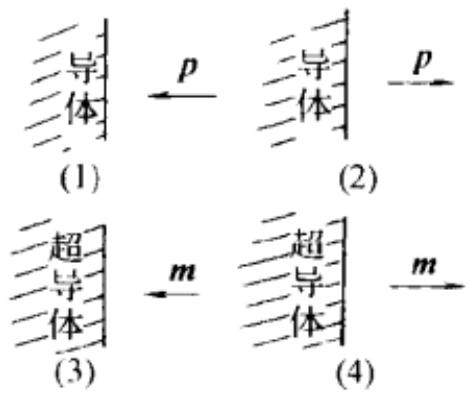
\includegraphics[width=0.5\linewidth]{figures/fig_8_4_4_1.jpg}
\end{center}
\begin{center}
    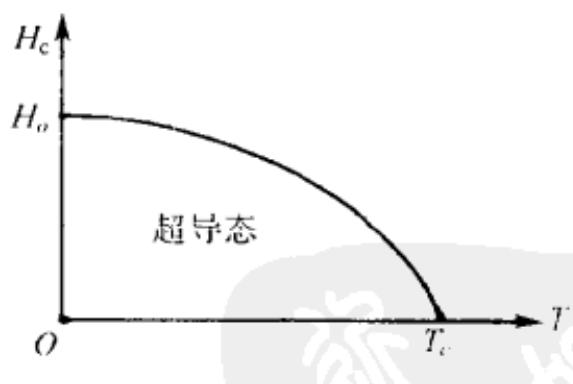
\includegraphics[width=0.5\linewidth]{figures/fig_8_4_4_2.jpg}
\end{center}

\vfill

\newpage

\textbf{8.4.5.} 超导材料在温度 $T < T_{c}$ (临界温度) 时处在超导态, 这时如有电流通过它, 在它的表面上产生的磁场强度 $H > H_{c}$ , 超导态就会被破坏. $H_{c}$ 称为临界磁场. 实验得出, $H_{c}$ 与温度 T 的关系为

$$
H _ {\mathrm{c}} = H _ {0} \left[ 1 - \left(\frac {T}{T _ {\mathrm{c}}}\right) ^ {2} \right]
$$

式中 $H_{0}$ 是 T=0 时的临界磁场。(1)以 T 为横坐标, $H_{c}$ 为纵坐标, 画出 $H_{c}-T$ 曲线, 并标明超导态的区域; (2)铅的 $T_{c}=7.2K, H_{0}=6.39\times10^{4}A/m$ , 试问用铅做成半径为 1.0mm 的导线, 在 T=3.6K 时能通过多大的电流而不破坏超导态?

\vfill

\textbf{8.4.6.} 半径为 R 的超导圆环, 自感为 L, 放在磁感强度为 B 的均匀磁场中, 环的轴线与 B 垂直, 环内没有电流. 现将这环绕垂直于 B 的直径转 $90^{\circ}$ , 使它的轴线平行于 B. 试求: (1) 环内的电流 I; (2) 外力作的功.

\vfill

\newpage

\textbf{8.4.7.} 用横截面半径为 $a = 1.0\mathrm{mm}$ 的超导线做成圆环，环的半径为 $R = 25.0\mathrm{mm}$ . 在温度高于临界温度 $T_{\mathrm{c}}$ 时，将这圆环放在磁感强度为 $\pmb{B}$ 的均匀磁场中，圆环的轴线与 $\pmb{B}$ 平行，环内电流为零. 然后将温度降低到 $T_{\mathrm{c}}$ 以下，再撤去磁场. 试求圆环中的电流. 已知 $B = |\pmb{B}| = 5.0\mathrm{Gs}$ ，圆环的自感为 $L = \mu_0 R (\ln \frac{8R}{a} - 1.75)$ .

\vfill
